\documentclass[a4paper,titlepage]{article}

\usepackage[utf8]{inputenc}
\usepackage{graphicx}
\graphicspath{ {images/} }

\usepackage[a4paper,top=2cm,bottom=2cm,left=2cm,right=2cm,marginparwidth=1.75cm]{geometry}
\usepackage{url}
\usepackage{xurl}
\usepackage{siunitx}
\usepackage{natbib}
\usepackage{graphicx}
\usepackage{pgfplots}
\usepackage{indentfirst}
\usepackage{amsmath}
\usepackage{amssymb}
\usepackage{hyperref}
\usepackage{authblk}
\usepackage{multirow}
\usepackage{booktabs}% http://ctan.org/pkg/booktabs
\newcommand{\tabitem}{~~\llap{\textbullet}~~}

\pgfplotsset{compat=1.17}

\setlength{\parskip}{1em}

\DeclareMathOperator{\arcsec}{arcsec}
\DeclareMathOperator{\arccot}{arccot}
\DeclareMathOperator{\arccsc}{arccsc}

\title{

\includegraphics[width=4cm]{sst.png}\\
\vspace{1cm}
\textbf{COVID-19 Advocacy}\\
{\large Secondary 3 Elementary Mathematics Performance Task}}

\author{Ryan Theodore The\thanks{ryan\_theodore\_the@s2019.ssts.edu.sg}}
\author{Koh Jieming Xavier\thanks{koh\_jie\_ming\_xavier@s2019.ssts.edu.sg}}
\author{Joe Wong\thanks{joe\_wong@s2019.ssts.edu.sg}}
\affil{School of Science and Technology, Singapore}

\date{\today}

\begin{document}

\maketitle

{\setlength{\parskip}{0pt}\tableofcontents}

\pagebreak
\section{Introduction}\label{sec:Introduction}

\subsection{Learning Goals}

To understand how the number of COVID-19 cases would increase without safety measures by mapping the number of COVID cases as an exponential function. Students are to decide on an appropriate exponential function to map and predict the number of COVID cases if no measures are taken.

\subsection{Role}

You are a team of youth ambassadors who want to educate the public, in particular, students, about the importance of mandatory mask wearing and Safe Measurement Measures (SMM) in curbing the spread of the COVID-19 virus.

\subsection{Audience}

Your audience are the students of the school. 

\subsection{Situation}

As seen in the news, there are still members of the public who are still not wearing masks or adhering to the Safe Measurement Measures (SMM) like seen in Figure \ref{fig:noSmm}.

\begin{figure}[htbp]
    \centering
    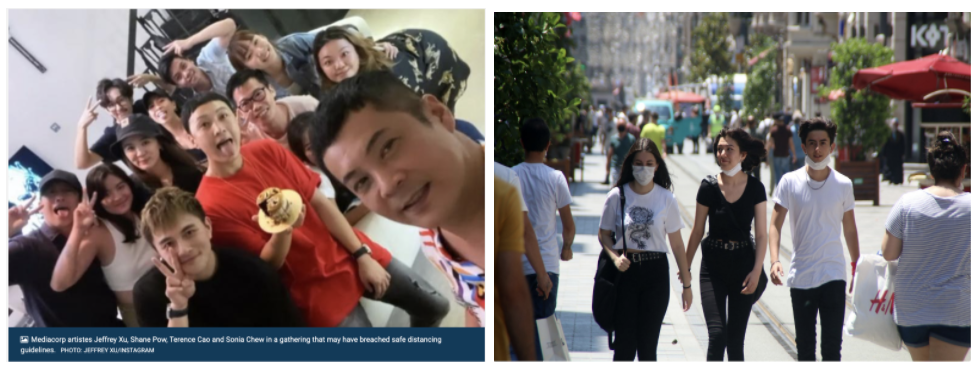
\includegraphics[width=7cm]{noSmm.png}
    \caption{People not obeying the Safe Measurement Measures (SMM) for the prevention of COVID-19}
    \label{fig:noSmm}
\end{figure}

\subsection{Task}

Your task is to educate students of your school to have a greater awareness of the importance of wearing masks and following safe management measures (SMM) so that they can influence their family members to do so as well. You are to approach this mathematically by modelling the number of infected cases in Singapore and up to two other countries using an exponential function. For instance, you can use the function, $y=ka^t$ or $y=ke^t$, in your explanation and presentation.

\subsection{Problem Statement}

To find a suitable graph to model the COVID-19 pandemic infection rate, in hopes of advocating to students in the School of Science and Technology, Singapore, and spreading awareness, on the importance of wearing masks and following the safe management measures.

\pagebreak
\section{Variables, Assumptions and Simplifications}

\subsection{Independent Variables}

\subsubsection{Wearing of Masks}

Wearing masks significantly reduces COVID-19 cases as tiny saliva droplets potentially loaded with viral particles, the main method that COVID-19 is spread, is blocked to a certain extent, based on the mask's effectiveness and whether or not both transmitter and receiver wear masks.

Assuming everyone wears a 50\% effective mask, there will be a 75\% drop in the chance of infection between people \cite{masksim_bhatia_2020} like seen in Figure \ref{fig:mask2Effectiveness}.

\begin{figure}[htbp]
    \centering
    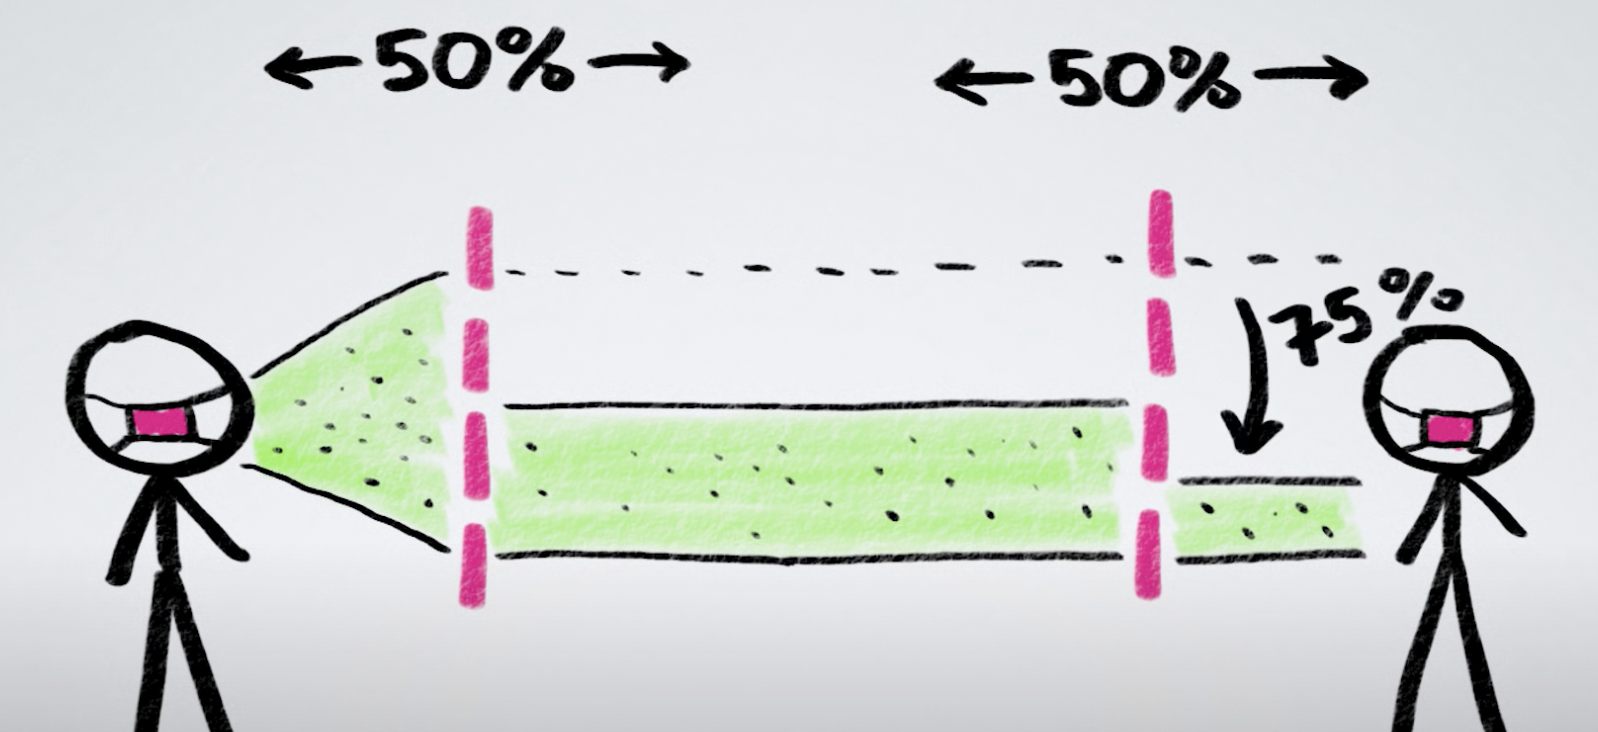
\includegraphics[width=7cm]{mask2Effectiveness.png}
    \caption{Effectiveness of masks when both transmitter and receiver wear masks, taken from \cite{maskvid_reich_2020}}
    \label{fig:mask2Effectiveness}
\end{figure}

Likewise, for the other 3 possible interactions between people, the drop in chance of infection for "NN", "YN", "NY", "YY", are 0\%, 50\%, 50\%, 75\%, respectively, where "N" represents a person who does not wear a mask and "Y" represents the inverse. This can been seen in Figure \ref{fig:maskAllEffectiveness}

\begin{figure}[htbp]
    \centering
    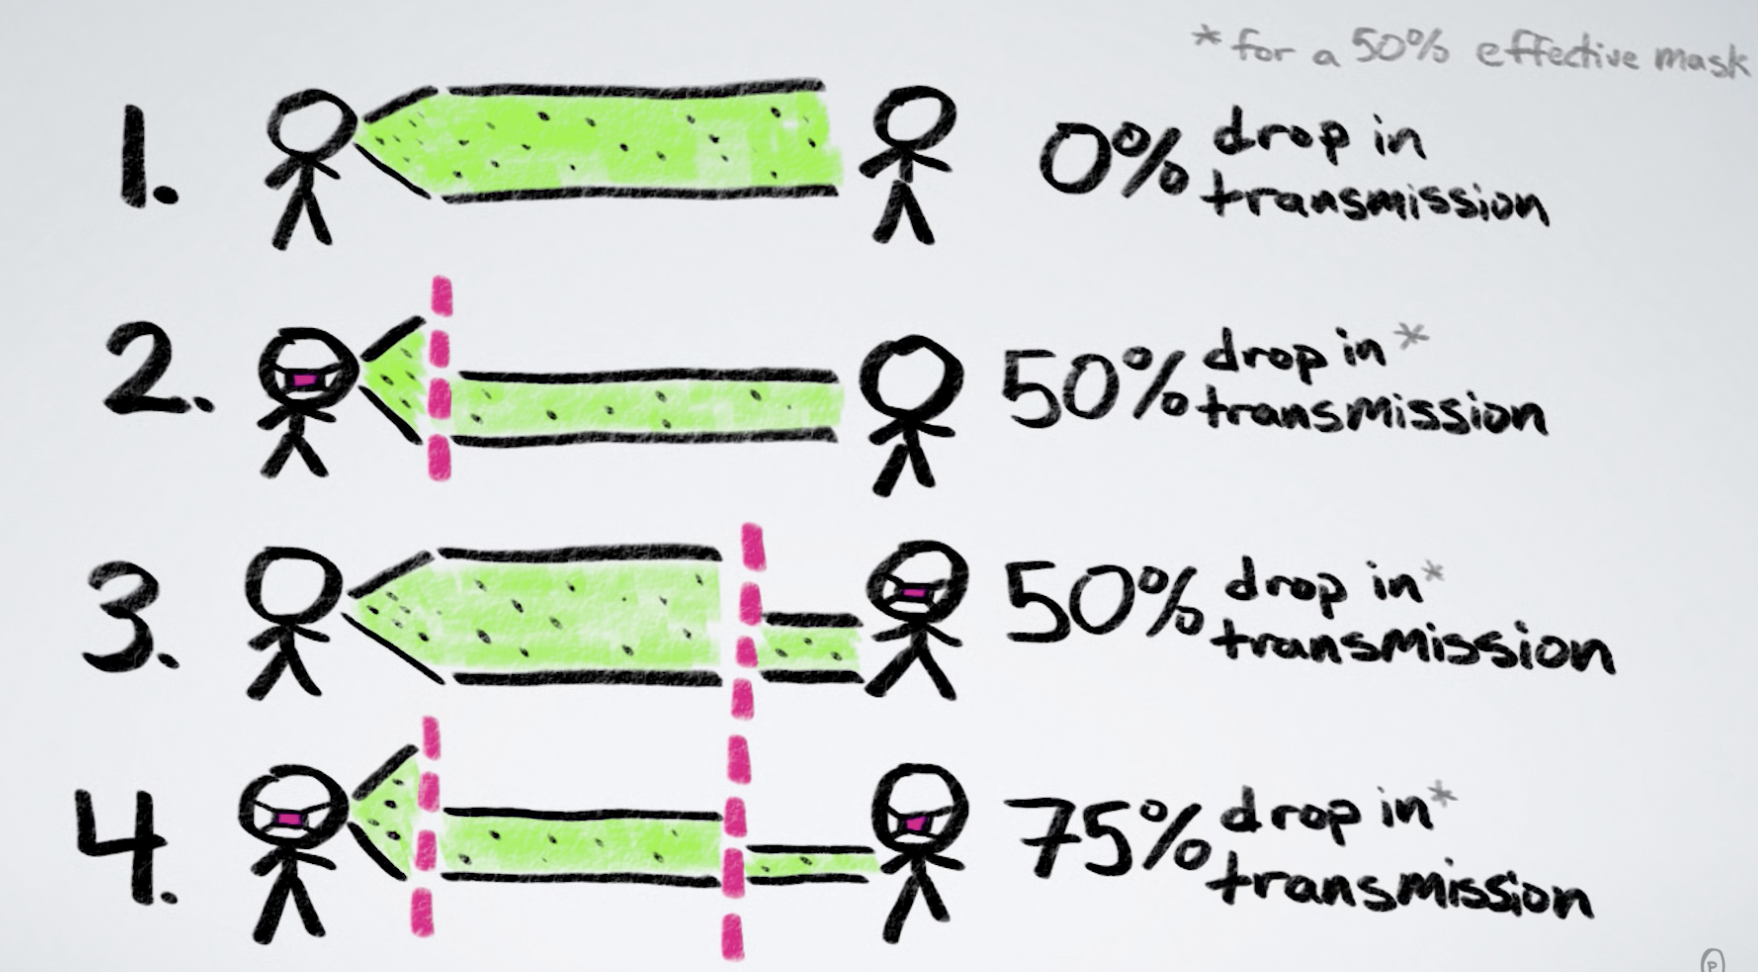
\includegraphics[width=7cm]{maskAllEffectiveness.png}
    \caption{Effectiveness of masks for various scenarios, taken from \cite{maskvid_reich_2020}}
    \label{fig:maskAllEffectiveness}
\end{figure}

Hence, although surgical masks are not as effective as the eponymous N95 masks (clearly supposedly 95\% effective), even masks that are 50\% effective, still greatly aid in lowering transmission rates.

\subsubsection{1m Social Distancing}

The term "social distancing" refers to the effort of people in keeping a certain distance apart from one another as much as possible. Thus, even with social distancing, it is still possible for contact and infections. This is because droplets are able to travel up to $2\si{m}$ \cite{droplets_setti_passarini_de_gennaro_barbieri_perrone_borelli_palmisani_di_gilio_piscitelli_miani_et_al_2020} when someone sneezes.

However, the percentage of the population that practices social distancing is still important. Social distancing can help reduce the number of droplets inhaled, as well as reducing the number of people a COVID-19 patient is exposed to.

Additionally, no matter how much one tries to avoid others, it is ultimately inevitable to come into contact of closer than the certain distance.

\subsection{Dependent Variables}

\subsubsection{Total number of COVID-19 infections}

The total number of COVID-19 infection cases on a given day changes depending on several factors including what day of the outbreak it is, $t$, and the number of infected cases on day $(t-1)$.

\subsubsection{Infection Rate and Chance}

The probability of an exposure becoming a new infection, $p$, depends on several determinants including whether people obey safe management measures of COVID-19 such as the wearing of masks and practising of social distancing.

A higher chance of infection will then increase the infection rate given a constant exposure rate.

\subsubsection{Social Exposure Rate}

The number of people that people are exposed to on a given day is affected by whether people stay home and practice social distancing.

\subsubsection{Growth Factor}

The growth factor refers to the percentage change in the number of cases. This value is given by the change in the number of cases on any given day, divided by the change in the number of cases the previous day. 

\subsection{Assumptions}

\subsubsection{COVID-19 Incubation Period}

According to the WHO, the incubation period of COVID-19 is 1 to 3 weeks, but most will have symptoms appear in 2 weeks. Thus, it is reasonable to assume that the time in days, $t$, before an exposed person knows if he or she is infected or not is 2 weeks, or $t=14$ \cite{incubation_who_2020}.

\subsubsection{People wearing Masks without removal}

It is assumed that people wear their masks and do not remove masks throughout the pandemic when in close contact with other people. Hence, this ensures that the transmission chances upon exposure is always applied.

\subsubsection{Isolated System of People}

It is assumed that people do not leave or enter the country, introducing and deporting cases, thus keeping an isolated system which is not affected by external causes.

\subsubsection{Infection Initial Case}

It is assumed that at the start of the pandemic, only 1 case of COVID-19 is introduced into the community rather than multiple cases.

\subsubsection{Immune after infection}

It is assumed that after a person has been infected and recovered from COVID-19, anti-bodies against the virus develops and thus the person is no longer susceptible to the virus and disease.

\subsubsection{Self-recovery Period}

It is assumed that people recover on their own gradually after the same amount of time regardless the person, not requiring sophisticated medical equipment at a hospital which would specifically increase gatherings at a location. 

\subsubsection{Movement (for simulation)}

It is assumed that no matter if a person is infected or not, they do not self quarantine at home and continues to move around freely. This models people leaving their homes for essential needs, which is a fundamental cause for the reason why cases do not converge to 0 albeit advanced contact tracing.

\subsection{Simplifications}

\subsubsection{Recovery Time}

According to BBC, the recovery time for the COVID-19 is at least 2 weeks \cite{recovertime_gallagher_2020}. To reduce the number of infected people at a given moment, which makes the great compound increase per day decrease, so as to not overemphasise the number of cases.

\subsubsection{Mask Types}

Different mask types worn by different people have different mask effectiveness rates which would affect the results of this model.

To ensure that the results of this model are not biased by using more effective or less effective mask types, a fair mask needs to be used.

Thus, to simplify the problem, it is reasonable to assume the masks used are fair masks with a effectiveness rate of 50\%.

\subsubsection{Herd Immunity}

Herd immunity, also known as population immunity, is the indirect protection from an infectious disease that happens when a population is immune either through vaccination or immunity developed through previous infection \cite{herdimmunity_who_2020}.

\subsubsection{Strain of Virus}

It is assumed that the COVID-19 virus represented in the simulations are of the same strain, hence having the same infection rates, recovery rates, and overall characteristics.

\pagebreak
\section{Mathematical Model}

Note: All graphs and functions in this section is plotted using Desmos. Our document can be found at \url{https://www.desmos.com/calculator/9a1kd4aghu}

Using data gathered from online, which will be presented below, estimations and predictions can be made on future cases, and different scenarios where people act differently. 

For instance, what if people did not obey the mandatory social distancing law? What if people did not wear masks? What if people completely ignored the fact that COVID-19 existed and went on with their daily lives?

Those are the questions aimed to be answered in this mathematical model, ultimately utilising a mathematical function to model the growth of COVID-19 cases.

Hence, the answers can then be used to advocate for reasons that people should in fact follow the safe management measures put in place by health authorities.

\subsection{Number of Infection Function}

In order to find a suitable graph for the number of infections with respect to time in an epidemic, real data will be required.

\subsubsection{Concatenated Linear Segments}

Clearly, the number of infections increase and then level off after some time. Taking data from Singapore's COVID-19 infection rates \cite{covidsg_who_2021}, the infection rate began to level off around August 6, $t=195$, with $54,254$ cases.

Hence, the simplest graph that can be plotted for number of infections, $y$, against time in days, $t$, is a linear graph, $f_1(t,t_2)$, where $t_2$ is $t$ at which infections begin to level off and increase at a constant rate. This can be seen in Figure \ref{fig:f1Linear}.

\begin{align}
    f_1(t,t_2)=\begin{cases} 
      \frac{54254}{195}t & \text{if }t\le t_2 \\
      \frac{54254}{195}t_2 & \text{if }t\ge t_2\\
   \end{cases}
\end{align}

\begin{figure}[htbp]
    \centering
    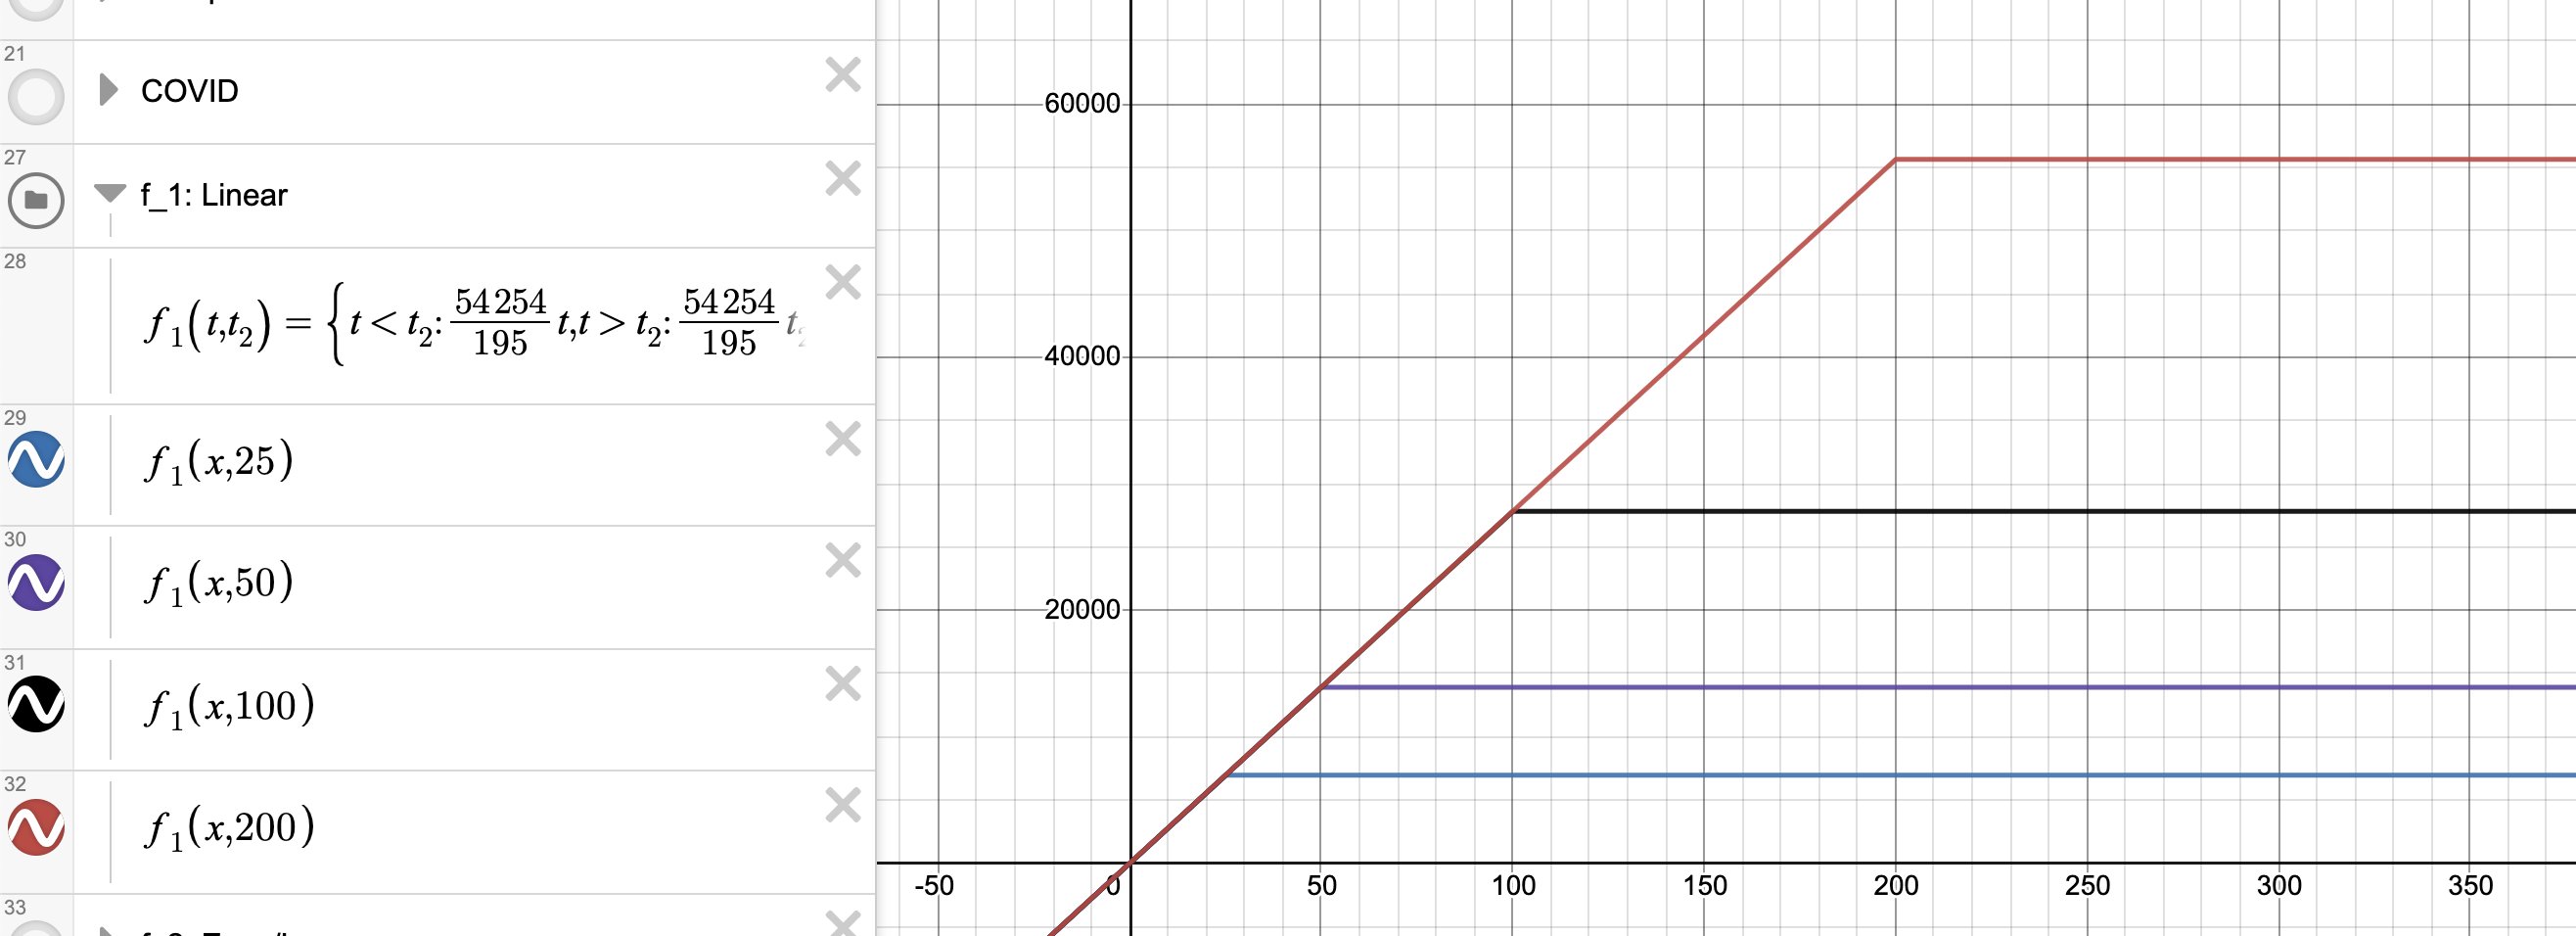
\includegraphics[width=10cm]{f1Linear.png}
    \caption{Concatenated Linear Segmented graph $f_1(t,t_2)$}
    \label{fig:f1Linear}
\end{figure}

\subsubsection{Concatenated Exponential and Logarithmic Segments}

Plotting a graph with only straight line segments and 2 plot points is surely highly inaccurate. The time at which the graph begins to turn from an exponentially increasing curve to one that increases slower, the inflection point, $t_1$, is not explicitly shown.

The segment between $t=0$ and $t=t_1$ can be modelled using an exponential graph. The segment between $t=t_1$ and $t=t_2$ can be modelled using a logarithmic graph. The segment $t>t_2$ can be modelled by a constant graph. Altogether, the piece-wise function, $f_2(t,t_1,t_2)$ is shown below, where $s$ is the sensitivity of implemented COVID-19 measures. This can be seen in Figure \ref{fig:f2ExpoLog}.

\begin{align}
    f_2(t,t_{1},t_{2},s)=\begin{cases}
        t^2 & \text{if }t\le t_{1} \\
        {t_1}^2+s\log\left(t-t_{1}+\frac{s}{400}\right)-s\log\left(\frac{s}{400}\right) & \text{if }t_{1}\le t+t_{1}\le t_{2}+t_{1}\\
        {t_1}^2+s\log\left(t_{2}-t_{1}+\frac{s}{400}\right)-s\log\left(\frac{s}{400}\right) & \text{if }t\ge t_{2}-t_{1}\\
   \end{cases}
\end{align}

\begin{figure}[htbp]
    \centering
    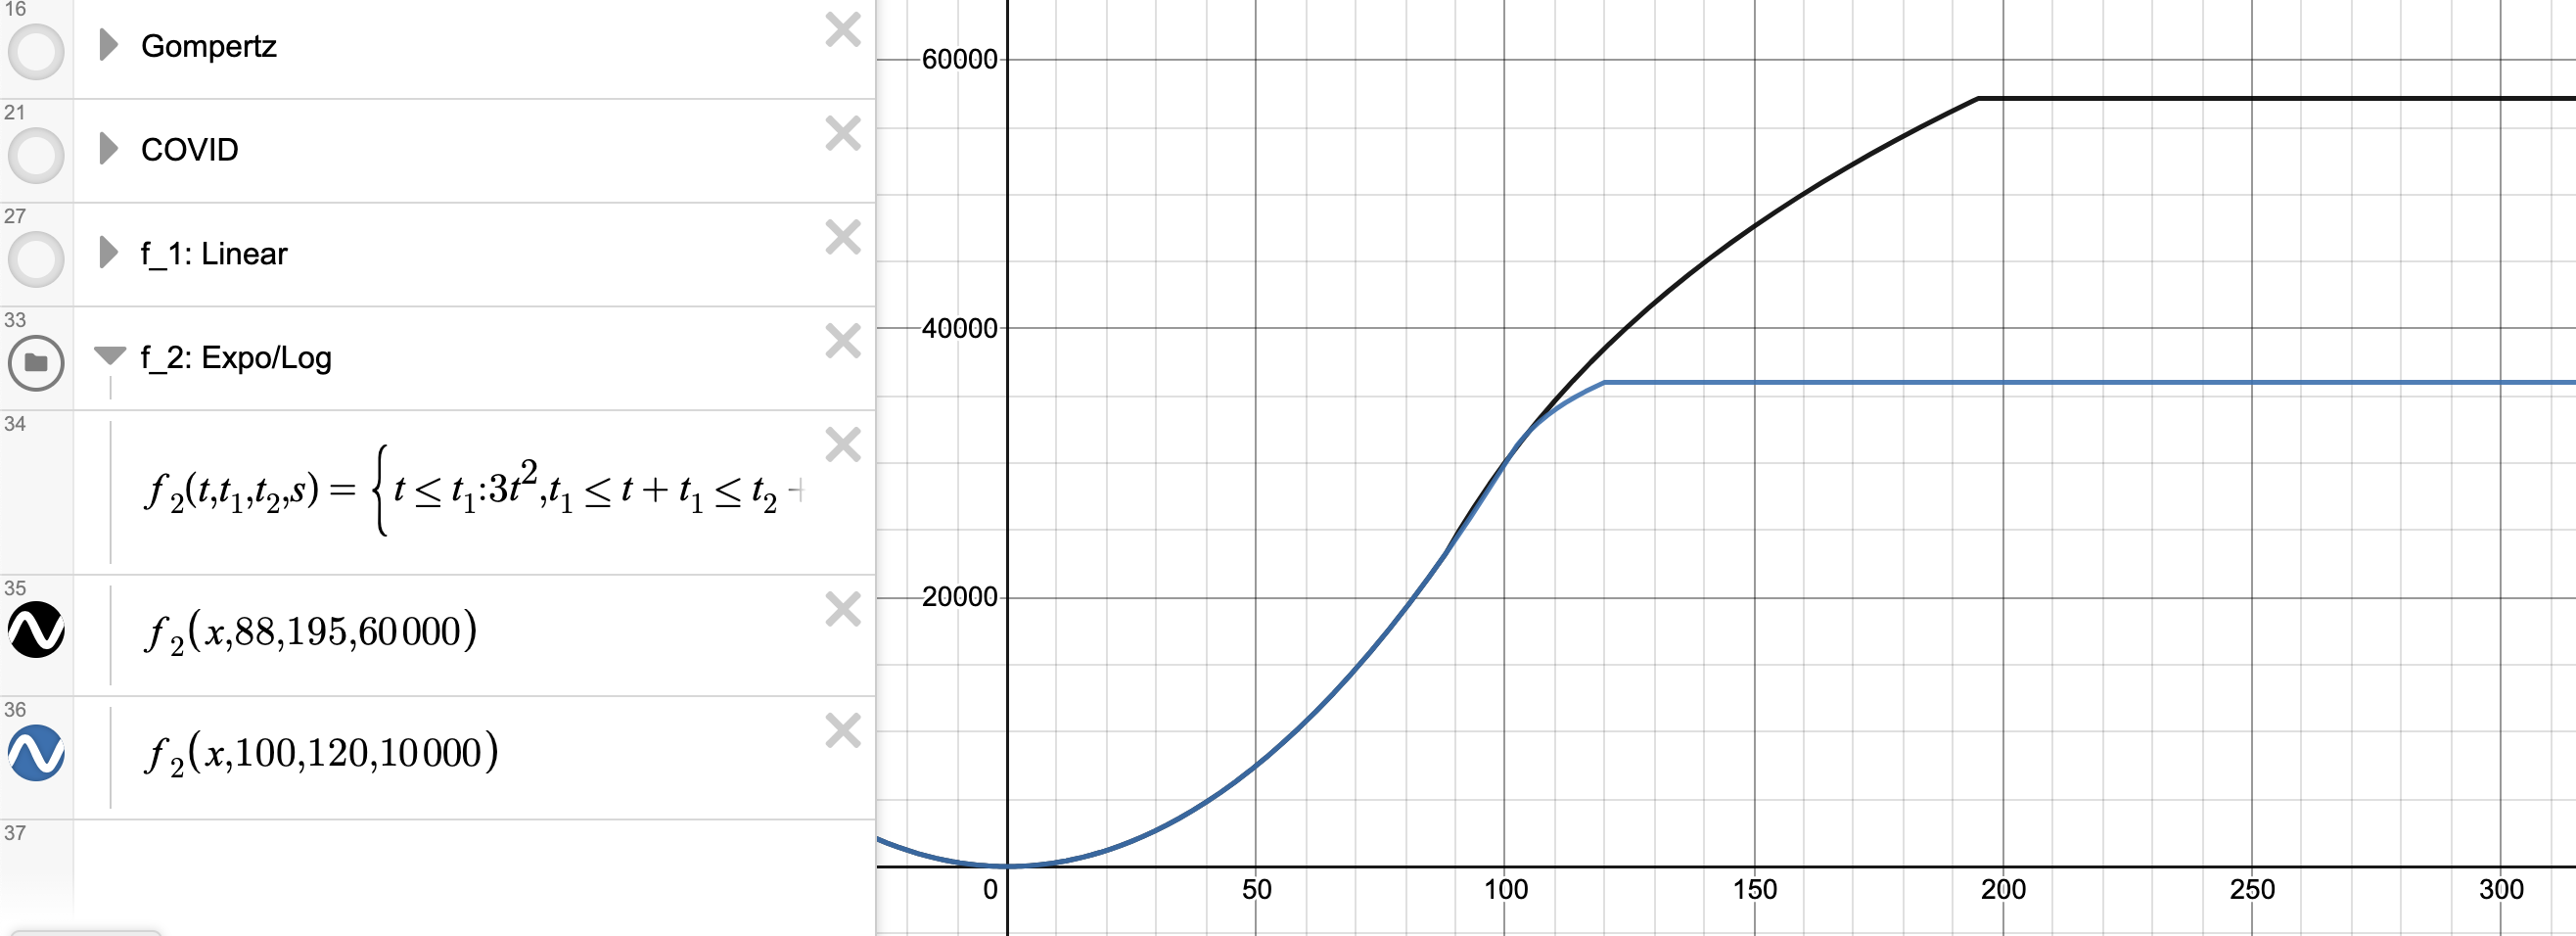
\includegraphics[width=10cm]{f2ExpoLog.png}
    \caption{Concatenated Exponential and Logarithmic Segmented graph $f_2(t,t_{1},t_{2},s)$}
    \label{fig:f2ExpoLog}
\end{figure}

\subsubsection{Combined Logistic and Gompertz Curves (Richards' Curve)}

However, our previous models can still be further improved with a Richards' Curve, also known as a generalised logistic function. This type of function is largely used in modelling epidemic infection trajectories including COVID-19 \cite{spreadcurves_lee_lei_mallick_2020}.

The improved model $f$ is shown below, where the flexibility of the curve is determined by $\xi$. In which if $\xi=1$ then the curve reduces to the logistic function, and if $\xi\to0$, then the curve converges to the Gompertz function. $\theta_1$, $\theta_2$ and $\theta_3$ represent the final epidemic size, infection rate, and lag phase, respectively \cite{richard_wikipedia_2021}.

A Gompertz function is a sigmoid function which describes growth as being slowest at the start and end of a given time period, causing a ease in and ease out infection rate, modelled by $f(t)=a\mathrm {e} ^{-b\mathrm {e} ^{-ct}}$ \cite{gompertz_wikipedia_2021}.

A logistic curve is very similar but has a few differences including, that (i) the location of the inflection point is exactly halfway between the two asymptotes and (ii) there is a radial symmetry in relation to the point of inflection \cite{logistic_10.2307/2347021}.

The difference between this function and a regular logistic function is the initial increase rate of cases, which can be seen in Figure \ref{fig:covidVsBasicLogistic}, where the red line is a normal logistic graph of the form $\frac {L}{1+e^{-k(x-x_{0})}}$, and the green line is $f_3(t,\theta_1,\theta_2,\theta_3,\xi)$.

\begin{figure}[htbp]
    \centering
    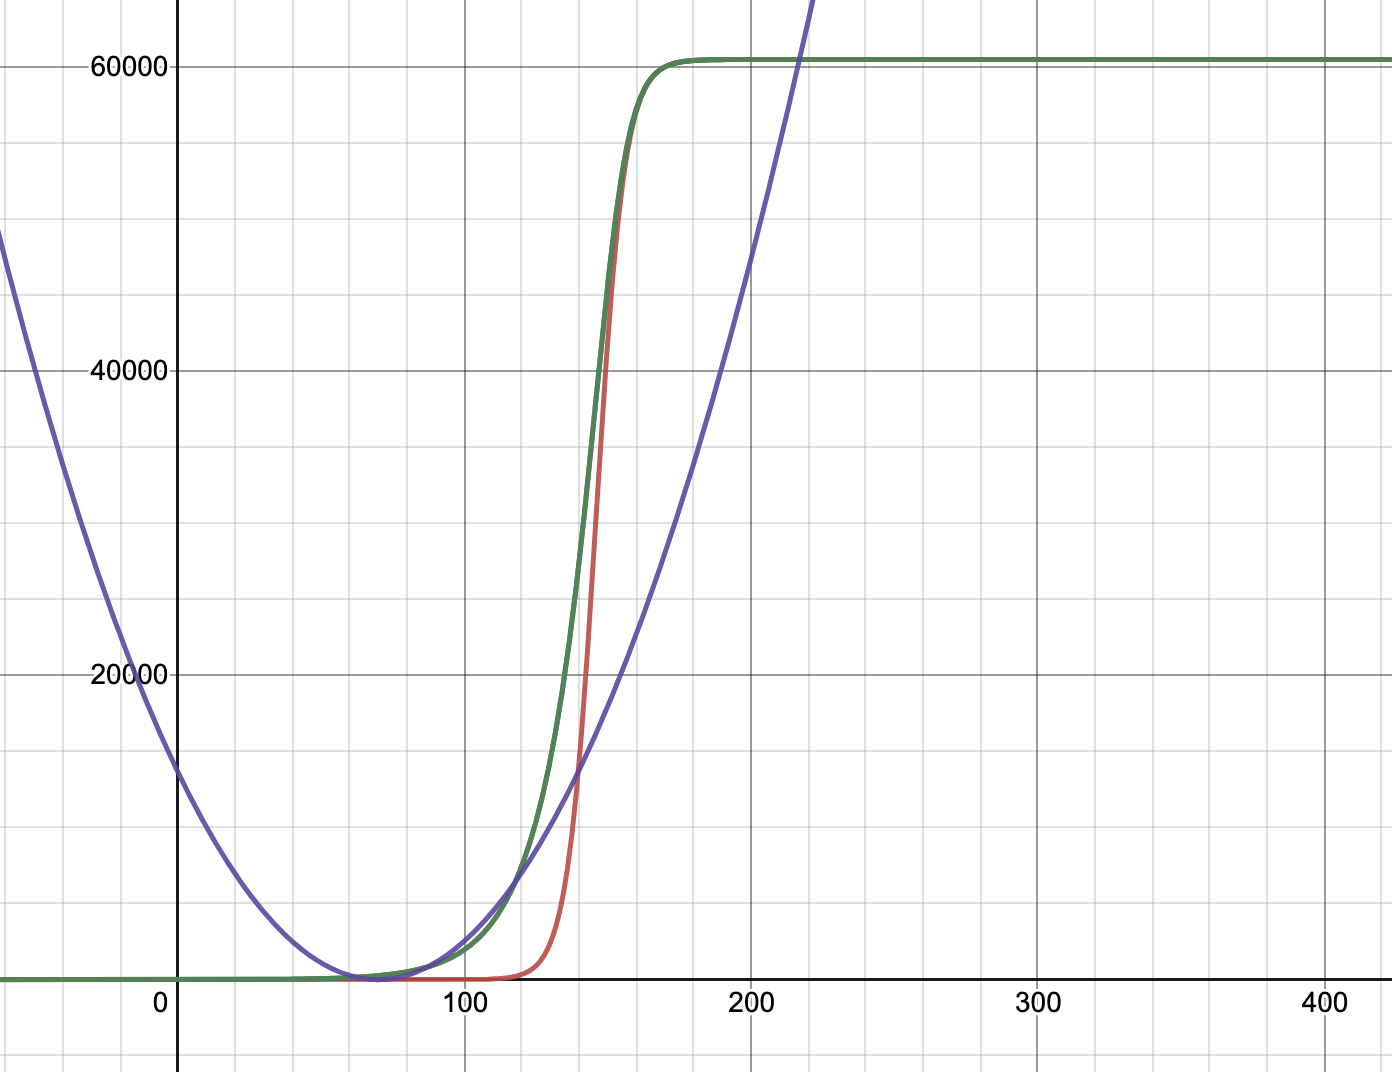
\includegraphics[width=10cm]{covidVsBasicLogistic.png}
    \caption{Difference between typical logistic curve and $f_3(t,\theta_1,\theta_2,\theta_3,\xi)$}
    \label{fig:covidVsBasicLogistic}
\end{figure}

\begin{align}
    f(t,\theta_1,\theta_2,\theta_3,\xi)={\frac {\theta _{1}}{[1+\xi \exp(-\theta _{2}\cdot (t-\theta _{3}))]^{1/\xi }}}
\end{align}

Singapore began implementing safe management measures on the 21 April, $t=88$

The characteristics of graph $f_3(t,\theta_1,\theta_2,\theta_3,\xi)$ are as follows, and seen in Figure \ref{fig:covidGraph}:

\begin{itemize}
    \item Initially, the graph is very similar to a exponential curve
    \item Eventually, the gradient decreases and becomes constant at the inflection point for some time
    \item Assuming no new clusters or outbreaks and continuous safe management measures, the infections should begin flattening and becoming constant
    \item However, if a cluster of outbreak does occur again, certain sections of the curve may repeat itself, with the worst being another exponential-like increase
\end{itemize}

\begin{figure}[htbp]
    \centering
    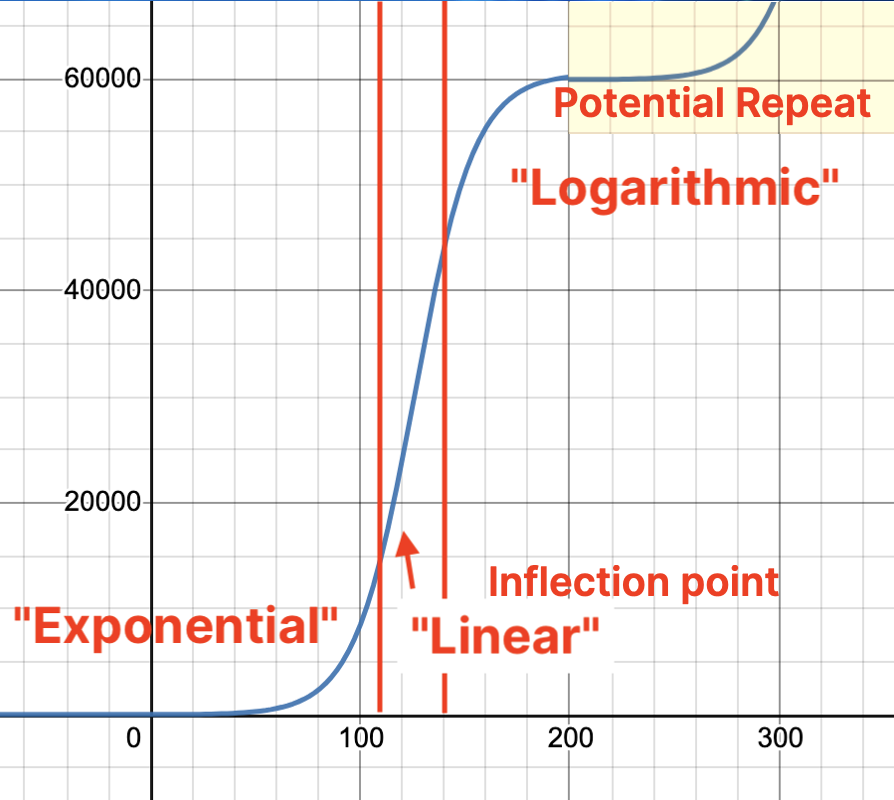
\includegraphics[width=10cm]{covidGraph.png}
    \caption{Characteristics of $f_3(t,\theta_1,\theta_2,\theta_3,\xi)$}
    \label{fig:covidGraph}
\end{figure}

\subsection{Data from Real World}

Utilising our model from above, the coefficient of regression, $R^2$, of the model can be calculated to find out the proportion of the variance in the dependent variable that is predictable from the independent variables. 

It is a statistic used in the context of statistical models whose main purpose is either the prediction of future outcomes or the testing of hypotheses, on the basis of other related information. It provides a measure of how well observed outcomes are replicated by the model, based on the proportion of total variation of outcomes explained by the model \cite{regression_draper_smith_1998}.

Essentially, $R^2$ gives numerical value to the accuracy of the model based off data. As $R^2$ approaches $1$, the accuracy of the model increases.

All data used in this section is attributed to the Center for Systems Science and Engineering (CSSE) at Johns Hopkins University, who has collected data from sites globally and collated it into a single repository \cite{globaldata_cssegisanddata_2021}, also recorded in the project data spreadsheet at \url{https://docs.google.com/spreadsheets/d/1qfm2fco4msClkVD8fAH6q-DRmDNM9yxGjrJtH5bGRzE#gid=159252991}.

Below is the graphs of the percentage of the people infected with COVID-19 against the time.

\subsubsection{Singapore}

Singapore recorded its first COVID-19 case on the 23 January 2020 \cite{covidtimeline_yong_2021}.

The country announced its nationwide partial lockdown, also known as the Circuit Breaker, that took effect on the 7 April 2020 \cite{covidlaw_ng_2020}. Citizens were required to stay in their place of residence unless absolutely essential such as purchasing supplies. The circuit breaker has surely led to a drop in the number of transmissions in Singapore.

Beginning 14 April 2020, the wearing of masks in public places in Singapore was made compulsory \cite{covidsg_who_2021}.

In view of the still increasing cases of COVID-19, the previously announced circuit breaker was extended to 1 June 2020 and measures were tightened, closing and restricting access to more services, causing citizens to stay home even more as less services are considered essential.

As part of Singapore's reopening after the circuit breaker, the Singaporean government made 1m social distancing mandatory and banned meetings in large groups. A contact tracing app called TraceTogether was also introduced to help health officials better quarantine close contacts to existing COVID-19 cases.

The tabulated real world data of Singapore can be found at \url{https://docs.google.com/spreadsheets/d/1qfm2fco4msClkVD8fAH6q-DRmDNM9yxGjrJtH5bGRzE#gid=2014796134}.

Singapore's infection count against days passed, $t$, together with the aforesaid function as a estimated trend line to the data, is plotted in Figure \ref{fig:rwG1}. The modelled function, $f_3(x,1,60519,0.07,126)$, has a coefficient of regression of $R^2=0.9609$.

\begin{figure}[htbp]
    \centering
    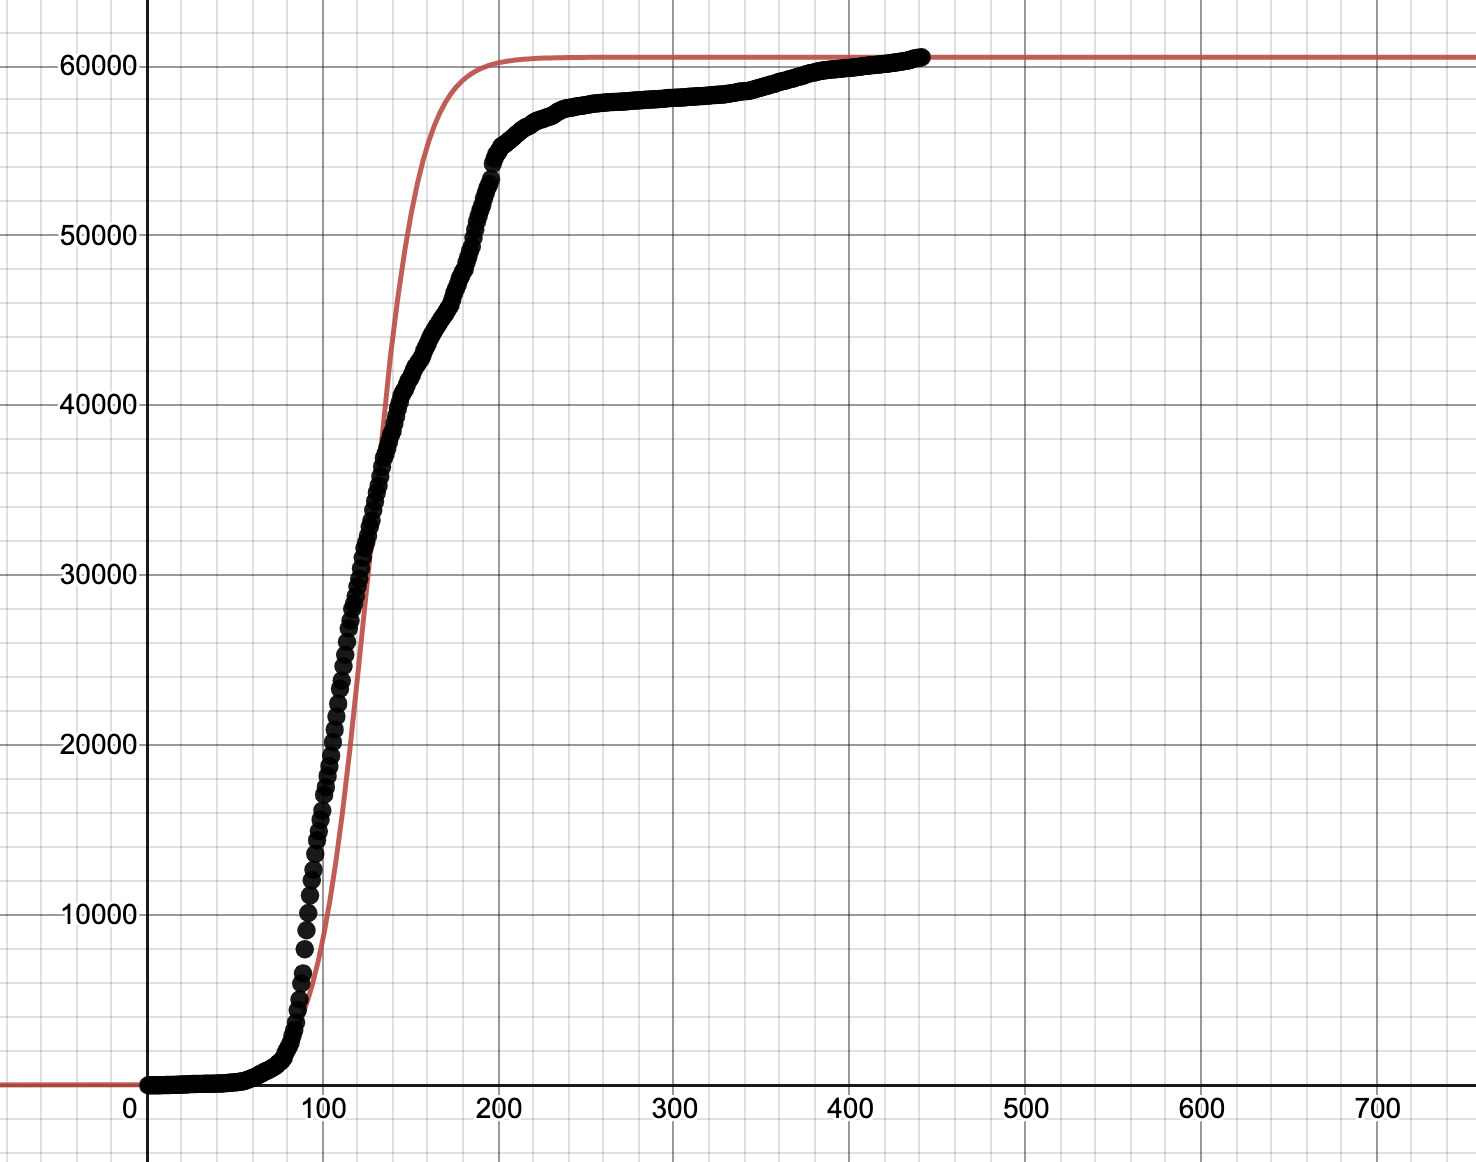
\includegraphics[width=10cm]{rwG1.png}
    \caption{Singapore's infection count with respect to days passed}
    \label{fig:rwG1}
\end{figure}

\subsubsection{India}

The Indian Ministry of Health and Family Welfare confirmed the first case of COVID-19 was on January 27 2020 in the southwestern coastal state of Kerala. 

On 24 March 2020, the Indian government declared a 21-day nationwide lockdown.

The cities in India are very densely packed and highly populated. Hence, many people find it hard to practice social distancing. India has a population of 1.3 billion people with a population density of 464 people per square kilometer \cite{indiadistance_pandey_2020}.

Especially because of the pandemic, many Indians are out of jobs and hence suffer from poverty. They are unable to afford their daily necessities and do not have enough to buy masks to wear.

The tabulated real world data of India can be found at \url{https://docs.google.com/spreadsheets/d/1qfm2fco4msClkVD8fAH6q-DRmDNM9yxGjrJtH5bGRzE#gid=628156050}.

India's infection count against days passed, $t$, together with the aforesaid function as a estimated trend line to the data, is plotted in Figure \ref{fig:rwG2}. The modelled function, $f_3(x,4,11046914,0.07,272)$, has a coefficient of regression of $R^2=0.9859$.

\begin{figure}[htbp]
    \centering
    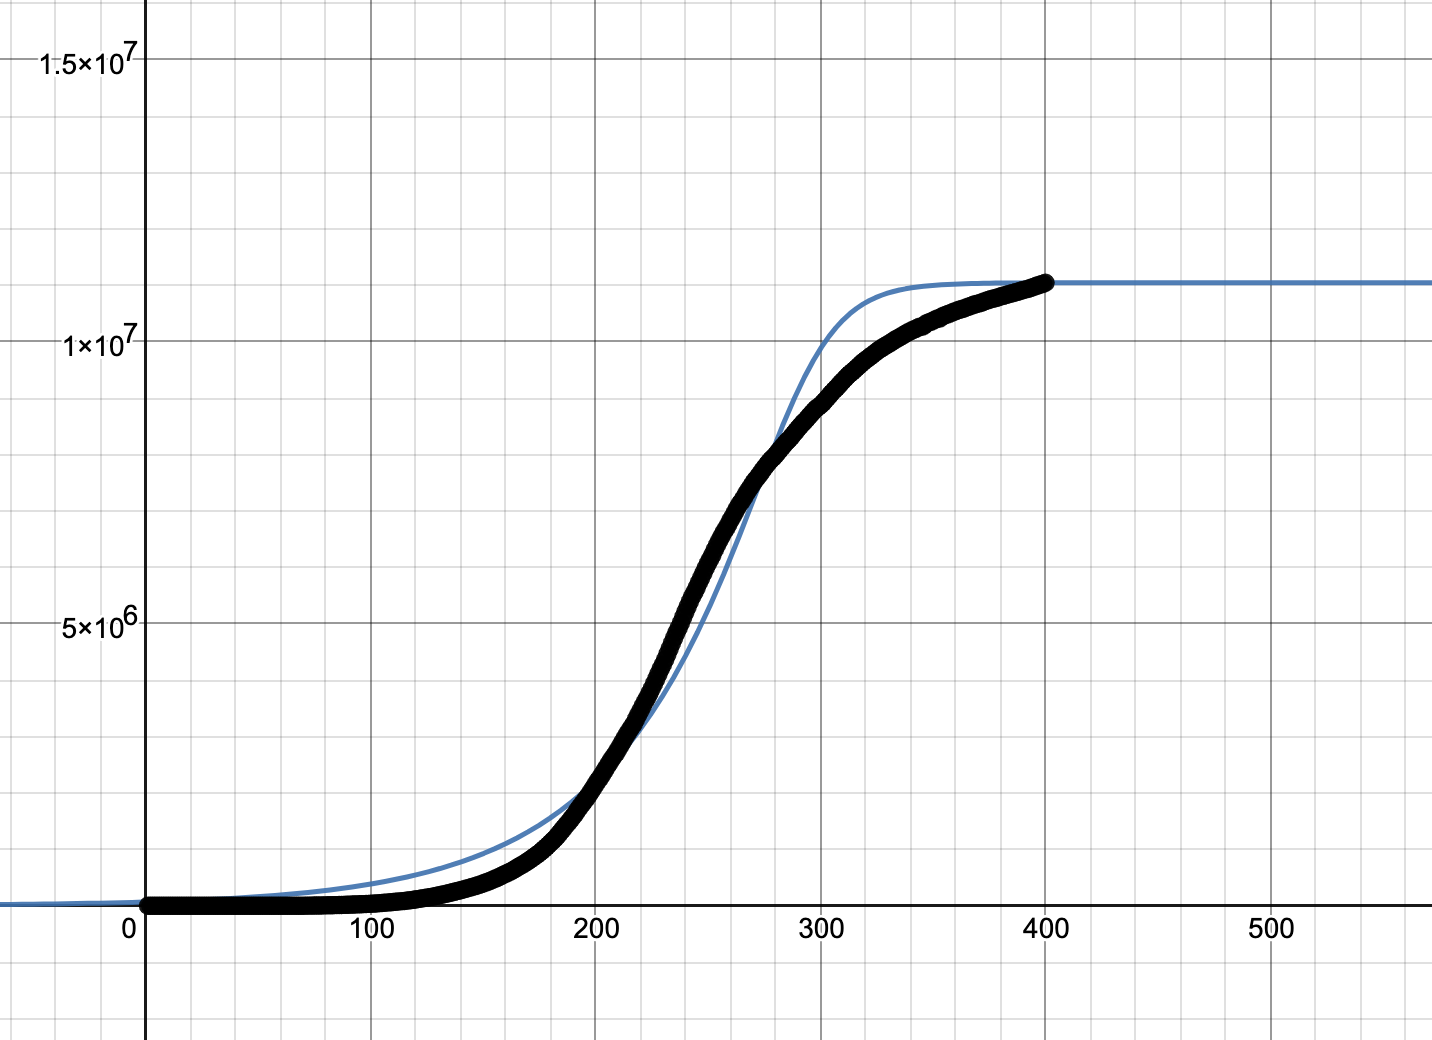
\includegraphics[width=10cm]{rwG2.png}
    \caption{India's infection count with respect to days passed}
    \label{fig:rwG2}
\end{figure}

However, in India, the number of cases after $t=400$ begins to increase seemingly exponentially yet again. This is an example of the repeating of this graph like seen in Figure \ref{fig:indiaRepeat}.

\begin{figure}[htbp]
    \centering
    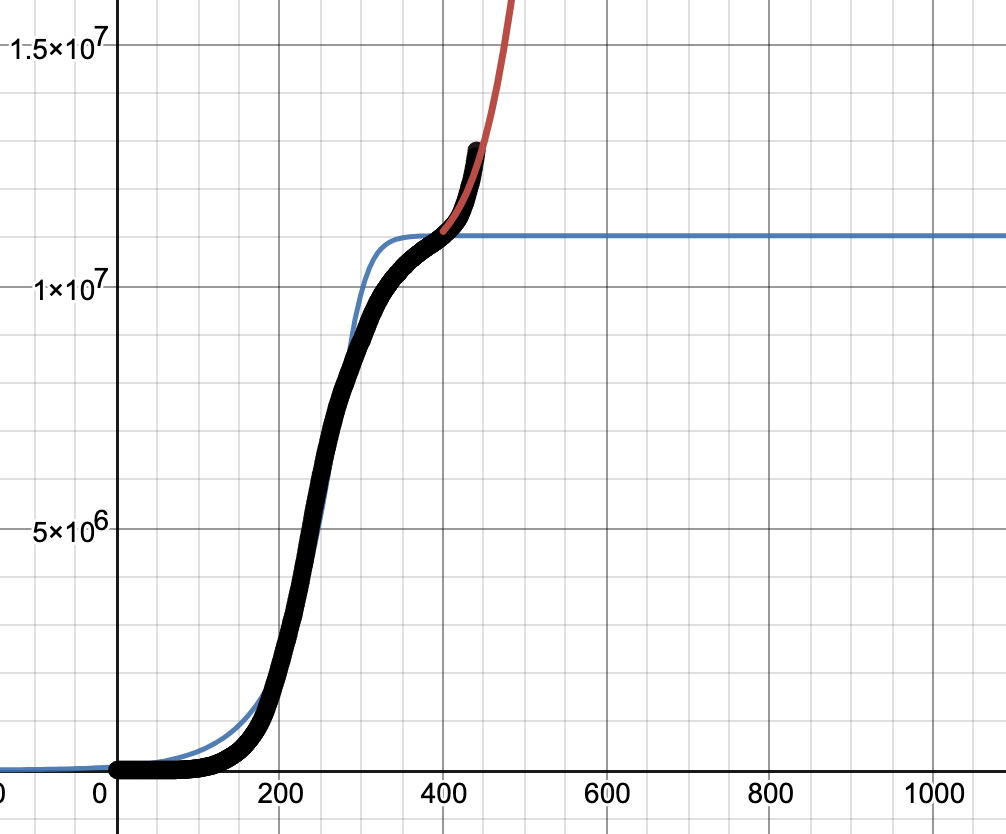
\includegraphics[width=10cm]{indiaRepeat.png}
    \caption{India's "repeating exponential curve"}
    \label{fig:indiaRepeat}
\end{figure}

\subsubsection{United States}

The first recorded case of COVID-19  in the United States was a Washington state resident on 21 January 2020. 

Over half the states in the US have mandates and laws that concern the wearing of masks.

The CDC recommends that US citizens maintain a safe distance of 1m when meeting up. However, some US residents ignore this recommendation and organise parties and go to clubs.

The US does not have a centralised system for contact tracing. Hence, healthcare workers are unable to isolate people who have been in close contact with COVID-19 cases, resulting in faster spreading of the virus.

The tabulated real world data of United States can be found at \url{https://docs.google.com/spreadsheets/d/1qfm2fco4msClkVD8fAH6q-DRmDNM9yxGjrJtH5bGRzE#gid=1880109553}.

United State's infection count against days passed, $t$, together with the aforesaid function as a estimated trend line to the data, is plotted in Figure \ref{fig:rwG3}. The modelled function, $f_3(x,5,30847348,0.07,350)$, has a coefficient of regression of $R^2=0.9885$.

\begin{figure}[htbp]
    \centering
    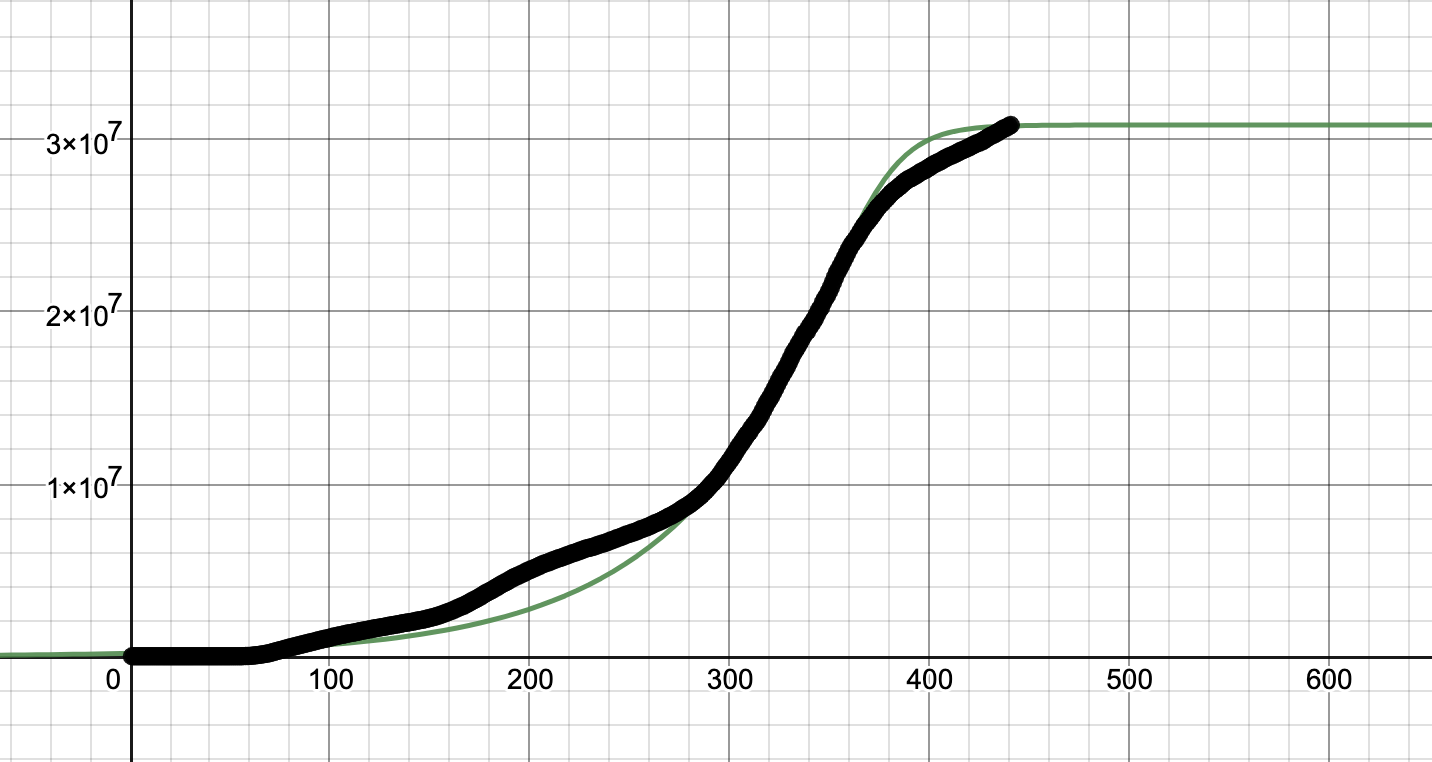
\includegraphics[width=10cm]{rwG3.png}
    \caption{United State's infection count with respect to days passed}
    \label{fig:rwG3}
\end{figure}

\subsection{Data from Simulation}

Apart from real world data where there are innumerable factors affecting the infection rate of COVID-19, simulations can also be utilised. By changing a single independent variable only, the single change in dependent variable would be conspicuous and intelligible easily.

In all the simulations, the constant parameters that are unchanged throughout the tests in experimentation process are that:

\begin{itemize}
    \item The original number of susceptible people = 100
    \item The original number of infected people = 1
    \item Recovery time of infected people in days = 14
    \item Movement speed in simulation units = 5 (actively moving)
\end{itemize}

\subsubsection{Base Case}

The established base case for the comparison is the simulation Test 1, with the variables below, can be seen in Figure \ref{fig:simT1}.

\begin{itemize}
    \item People do not wear masks, thus the transmission rate = $100\%$
    \item People do not social distance, thus distance apart = $0\si{m}$
\end{itemize}

\begin{figure}[htbp]
    \centering
    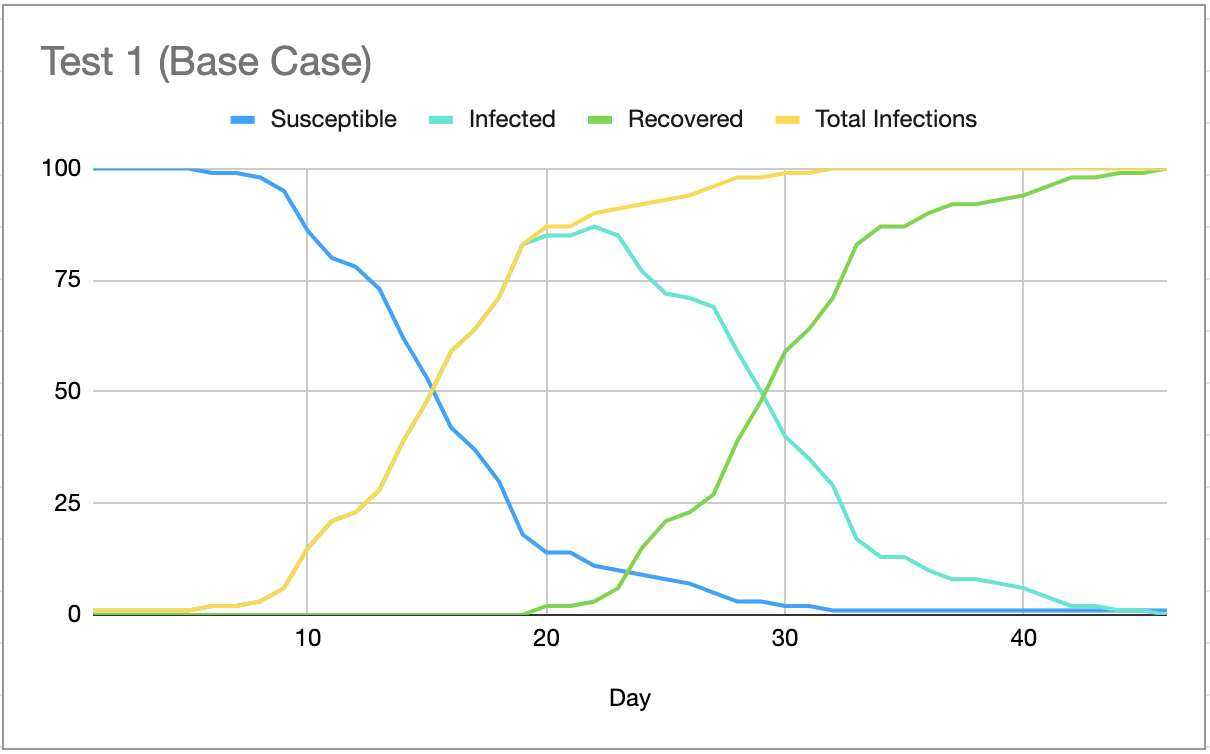
\includegraphics[width=10cm]{simT1.png}
    \caption{Best fit line of discrete points from Simulation Test 1}
    \label{fig:simT1}
\end{figure}

The video recording of Simulation Test 1 can be found at \url{https://drive.google.com/file/d/15WUWmvD2iKRdVvSlj1zRM-kNF0X1dRXr}, and the tabulated simulation data can be found at \url{https://docs.google.com/spreadsheets/d/1qfm2fco4msClkVD8fAH6q-DRmDNM9yxGjrJtH5bGRzE#gid=1160962421}.

Simulation Test 1's infection count against days passed, $t$, together with the aforesaid function as a estimated trend line to the data, is plotted in Figure \ref{fig:simG1}. The modelled function, $f_3(x,3.9,100,0.7,18)$, has a coefficient of regression of $R^2=0.9883$.

\begin{figure}[htbp]
    \centering
    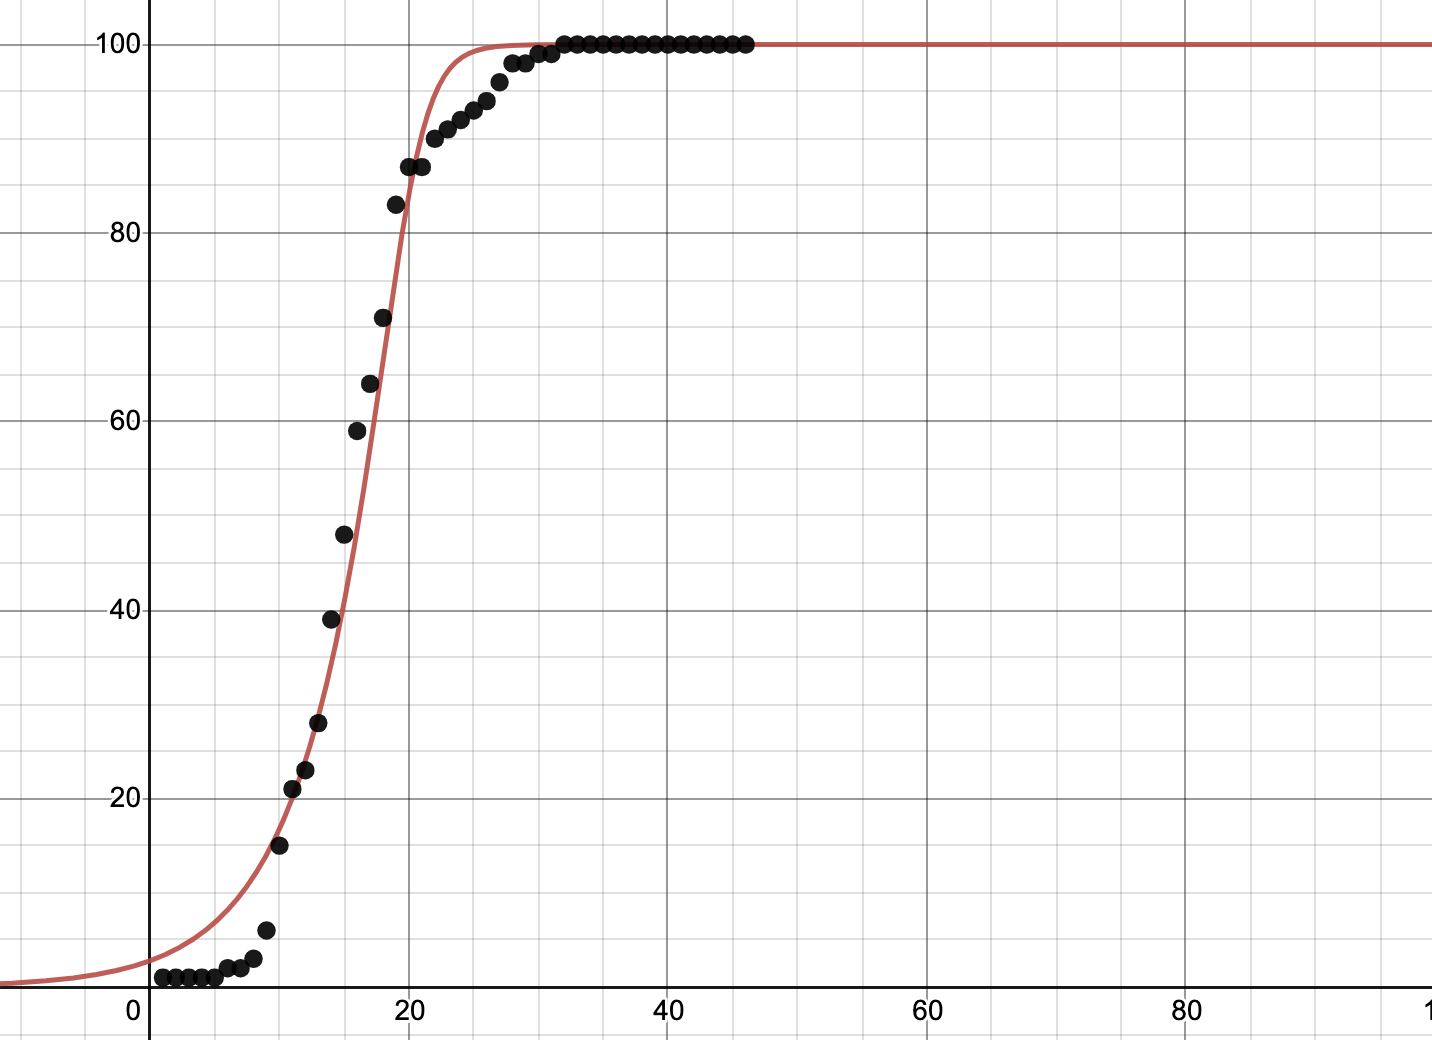
\includegraphics[width=10cm]{simG1.png}
    \caption{Simulation Test 1's infection count with respect to days passed, $f_3(x,3.9,100,0.7,18)$}
    \label{fig:simG1}
\end{figure}

\subsubsection{Wearing Masks}

When people wear masks, the simulation Test 2, with the variables below, can be seen in Figure \ref{fig:simT2}.

\begin{itemize}
    \item People wear masks, thus the transmission rate = $75\%$
    \item People do not social distance, thus distance apart = $0\si{m}$
\end{itemize}

\begin{figure}[htbp]
    \centering
    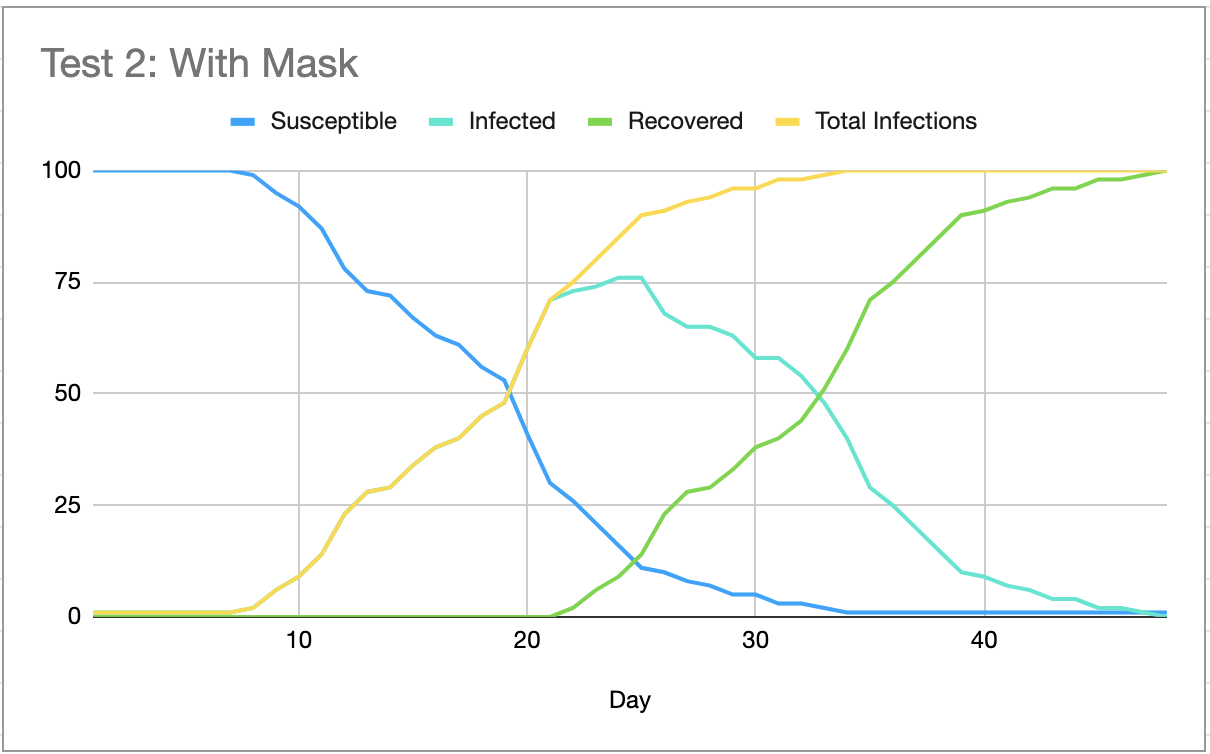
\includegraphics[width=10cm]{simT2.png}
    \caption{Best fit line of discrete points from Simulation Test 2}
    \label{fig:simT2}
\end{figure}

Between Test 1 to Test 2, the independent factor that was changed was the transmission rate, which resulted in a <u can leave this blank for graphing>. However, transmission rate is not the only factor that affects the infection rate, the social distancing also affects the infection rate.

The video recording of Simulation Test 2 can be found at \url{https://drive.google.com/file/d/1_-4P_fW3OhLt4wYZVEKffqGbMevf09o_}, and the tabulated simulation data can be found at \url{https://docs.google.com/spreadsheets/d/1qfm2fco4msClkVD8fAH6q-DRmDNM9yxGjrJtH5bGRzE#gid=1096946264}.

Simulation Test 2's infection count against days passed, $t$, together with the aforesaid function as a estimated trend line to the data, is plotted in Figure \ref{fig:simG2}. The modelled function, $f_3(x,3.9,100,0.6,21)$, has a coefficient of regression of $R^2=0.9925$.

\begin{figure}[htbp]
    \centering
    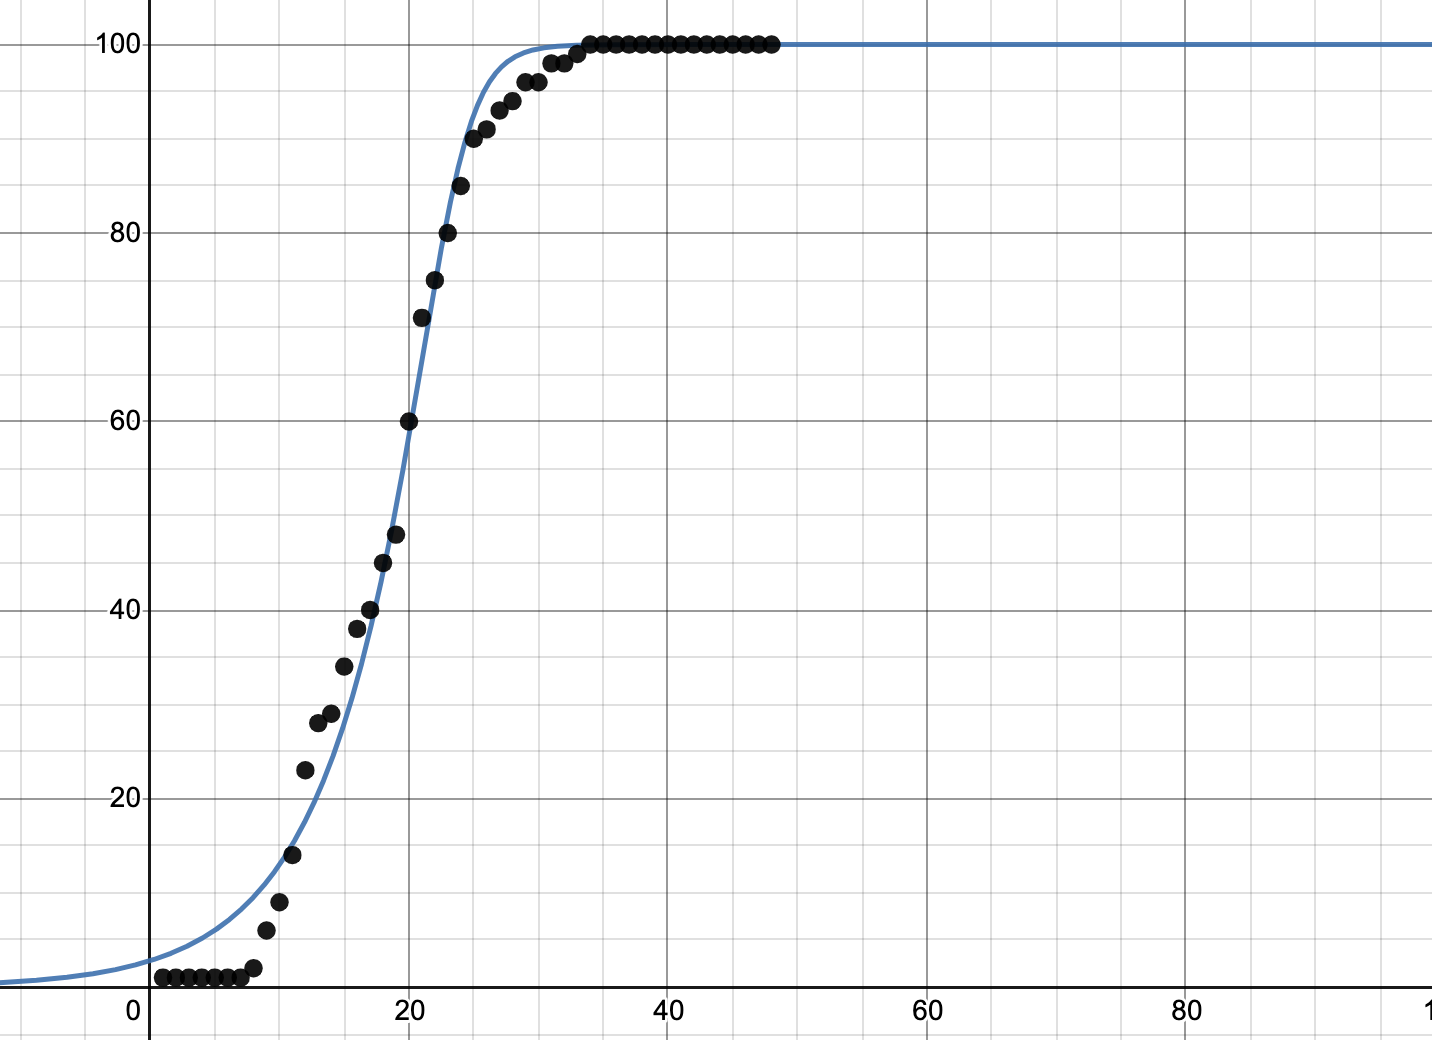
\includegraphics[width=10cm]{simG2.png}
    \caption{Simulation Test 2's infection count with respect to days passed, $f_3(x,3.9,100,0.6,21)$}
    \label{fig:simG2}
\end{figure}

\subsubsection{Social Distancing}

When people social distance, the simulation Test 3, with the variables below, can be seen in Figure \ref{fig:simT3}.

\begin{itemize}
    \item People do not wear masks, thus the transmission rate = $100\%$
    \item People social distance, thus distance apart = $1\si{m}$
\end{itemize}

\begin{figure}[htbp]
    \centering
    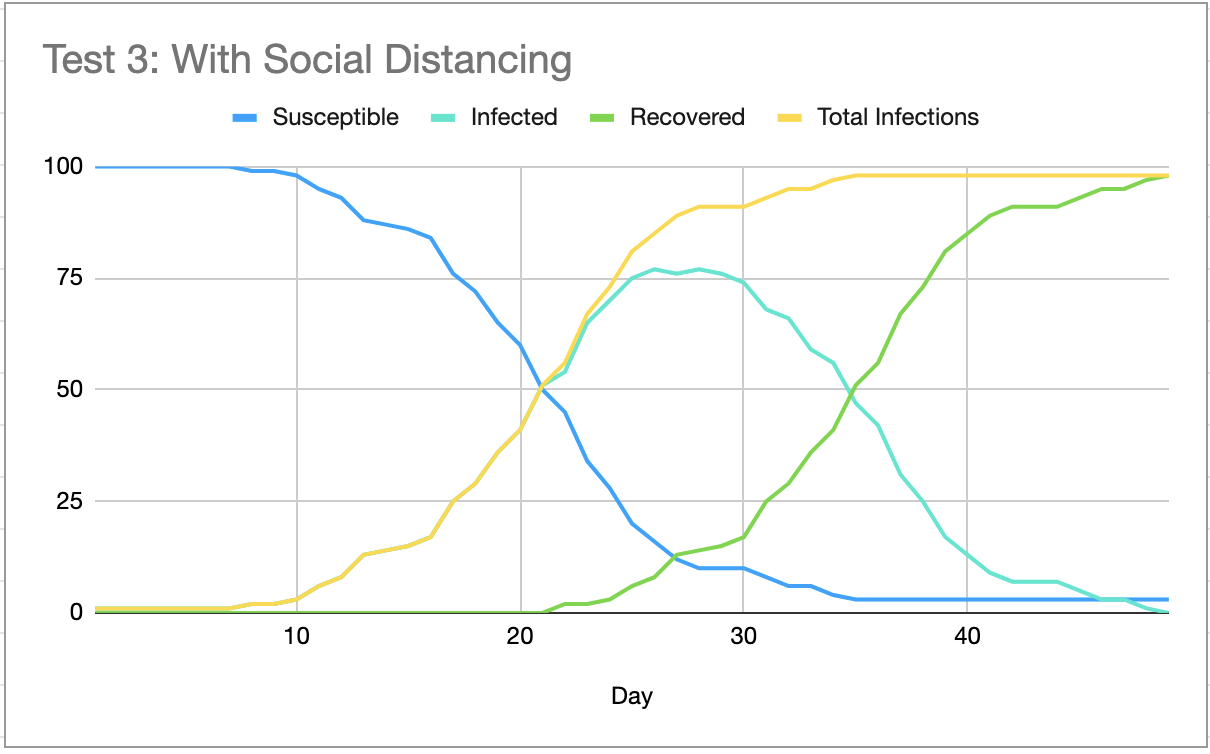
\includegraphics[width=10cm]{simT3.png}
    \caption{Best fit line of discrete points from Simulation Test 3}
    \label{fig:simT3}
\end{figure}

Between Test 1 to Test 3, the independent factor that was changed was the social distancing, which resulted in a <u can leave this blank for graphing>. However, social distancing is only one of the factors that affects the infection rate.

The video recording of Simulation Test 3 can be found at \url{https://drive.google.com/file/d/1E1eP3Dk-g7--2TGM0QGc4OsJHJED4tdj}, and the tabulated simulation data can be found at \url{https://docs.google.com/spreadsheets/d/1qfm2fco4msClkVD8fAH6q-DRmDNM9yxGjrJtH5bGRzE#gid=1841825833}.

Simulation Test 3's infection count against days passed, $t$, together with the aforesaid function as a estimated trend line to the data, is plotted in Figure \ref{fig:simG3}. The modelled function, $f_3(x,4,98,0.6,24)$, has a coefficient of regression of $R^2=0.9931$.

\begin{figure}[htbp]
    \centering
    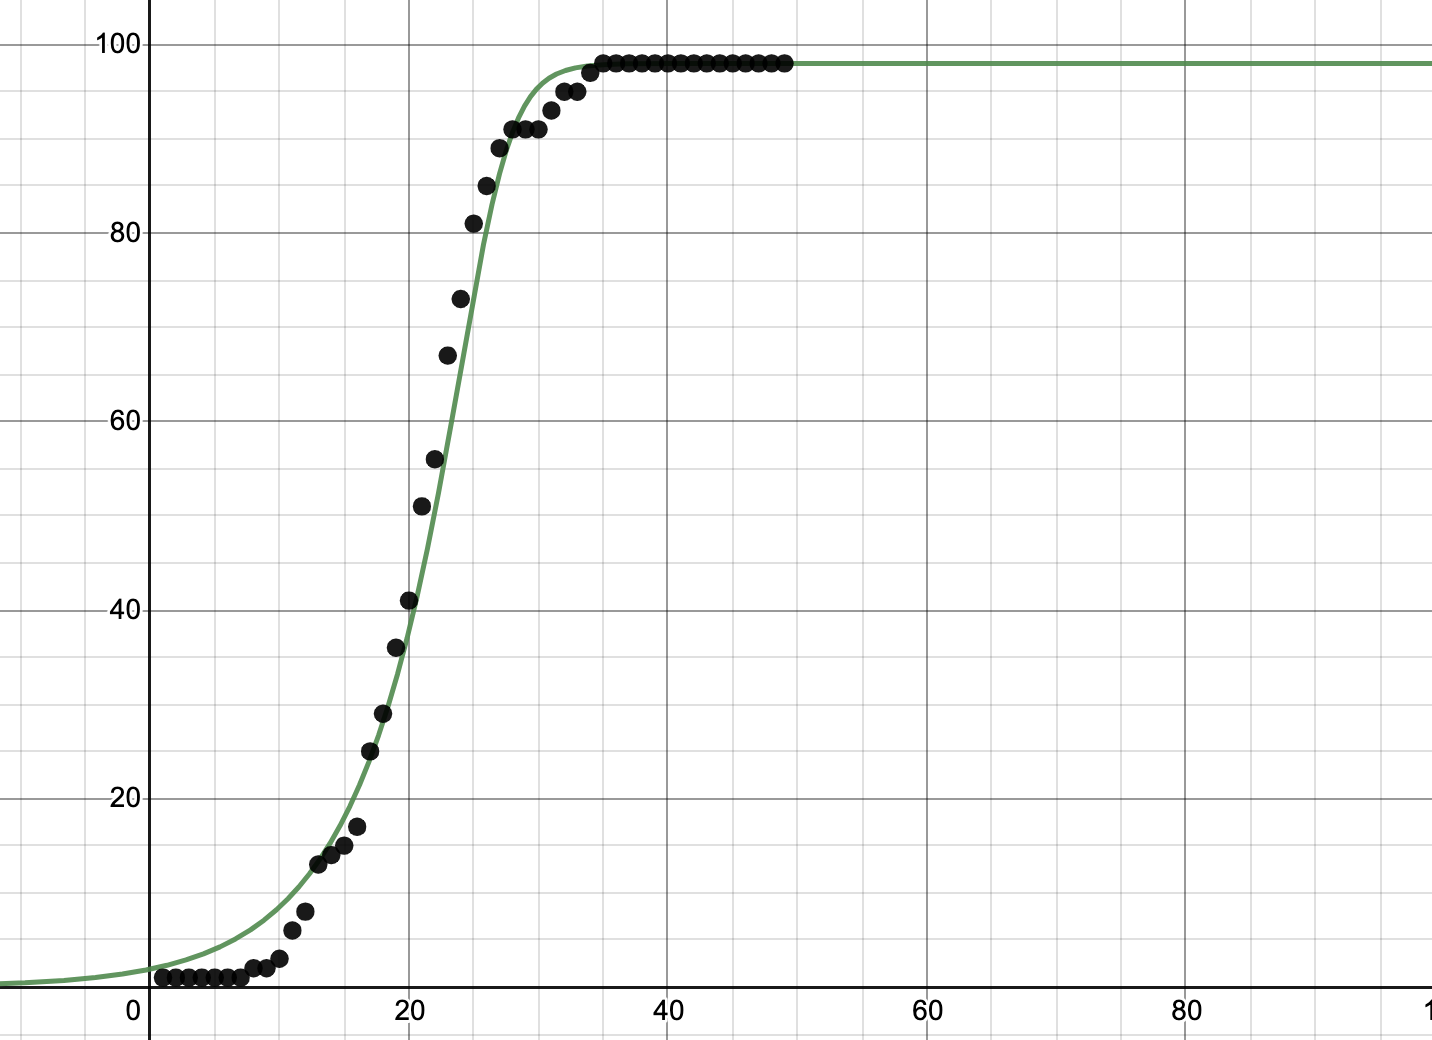
\includegraphics[width=10cm]{simG3.png}
    \caption{Simulation Test 3's infection count with respect to days passed, $f_3(x,4,98,0.6,24)$}
    \label{fig:simG3}
\end{figure}

\subsubsection{Both Social Distancing and Wearing Masks}

When people wear masks and social distance, the simulation Test 4, with the variables below, can be seen in Figure \ref{fig:simT4}.

\begin{itemize}
    \item People wear masks, thus the transmission rate = $75\%$
    \item People social distance, thus distance apart = $1\si{m}$
\end{itemize}

\begin{figure}[htbp]
    \centering
    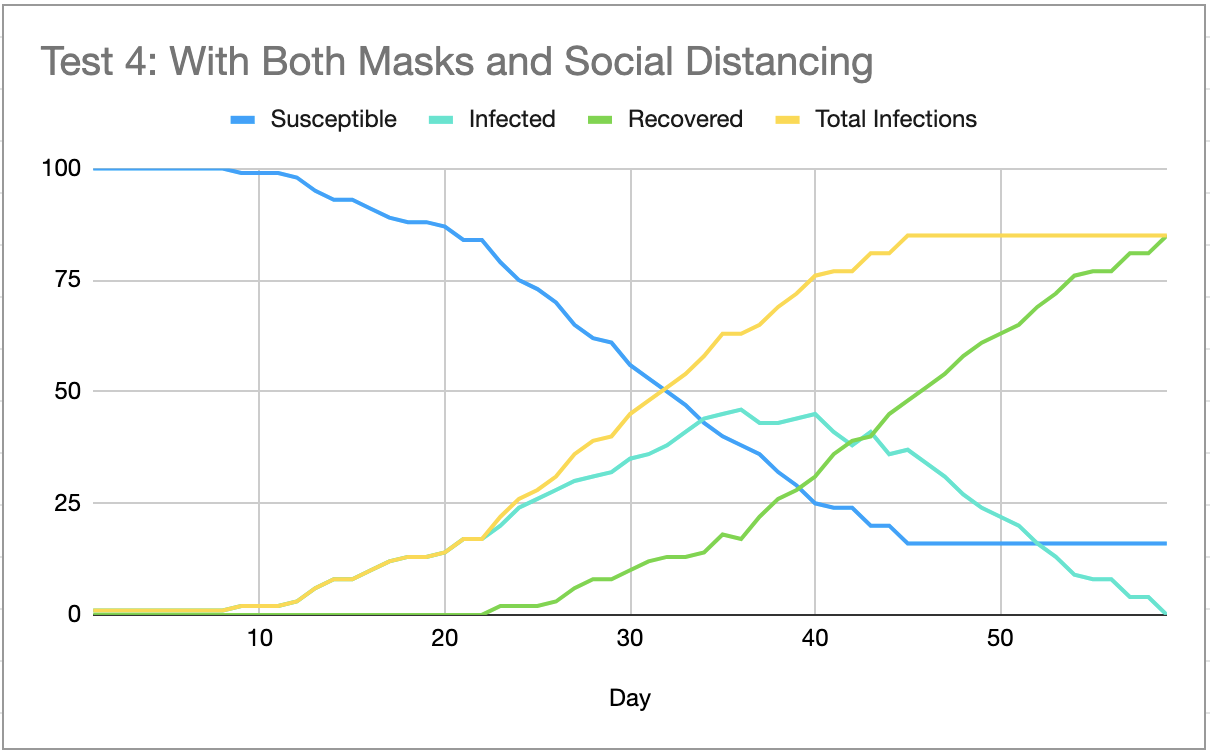
\includegraphics[width=10cm]{simT4.png}
    \caption{Best fit line of discrete points from Simulation Test 4}
    \label{fig:simT4}
\end{figure}

Between Test 1 to Test 4, the independent factor that changed was not only the transmission rate but also the social distancing, which resulted in a <u can leave this blank for graphing>. With both of the factors affecting the infection rate combined, the infection rate reduced significantly.

The video recording of Simulation Test 4 can be found at \url{https://drive.google.com/file/d/1tfN2vf3l8-HBvJKJcbNWporjqxNrnesq}, and the tabulated simulation data can be found at \url{https://docs.google.com/spreadsheets/d/1qfm2fco4msClkVD8fAH6q-DRmDNM9yxGjrJtH5bGRzE#gid=1542910455}.

Simulation Test 4's infection count against days passed, $t$, together with the aforesaid function as a estimated trend line to the data, is plotted in Figure \ref{fig:simG4}. The modelled function, $f_3(x,7.1,85,0.6,36)$, has a coefficient of regression of $R^2=0.9903$.

\begin{figure}[htbp]
    \centering
    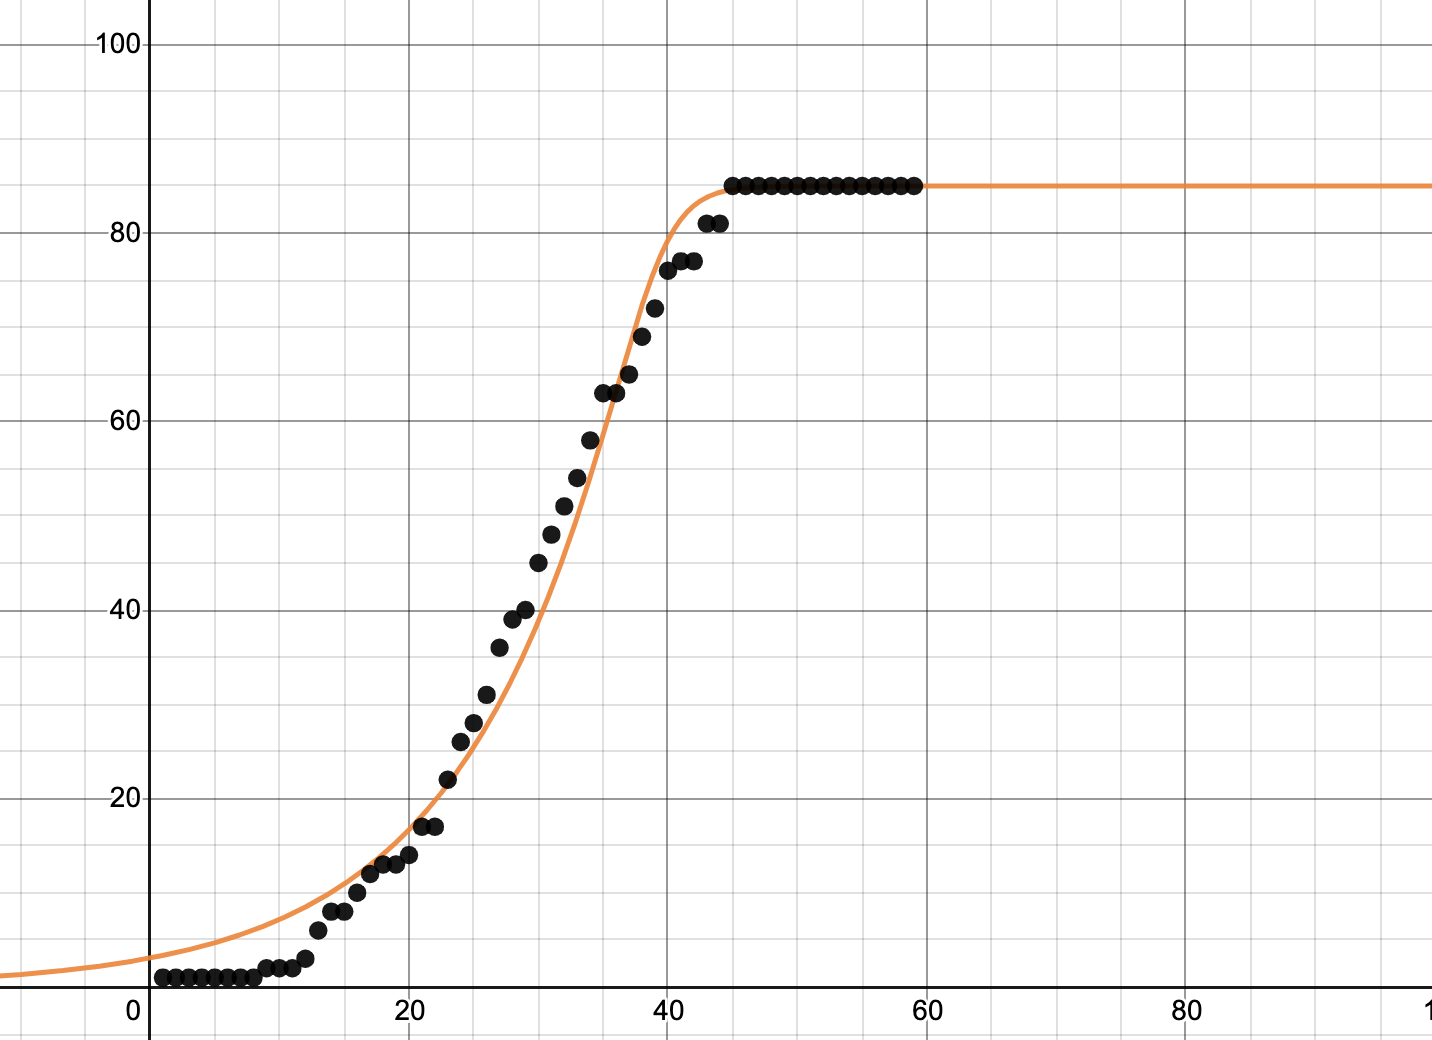
\includegraphics[width=10cm]{simG4.png}
    \caption{Simulation Test 4's infection count with respect to days passed, $f_3(x,7.1,85,0.6,36)$}
    \label{fig:simG4}
\end{figure}

\subsubsection{Summary}

In conclusion, both social distancing and the wearing of masks are necessary. In Test 4, the infection rate was much slower compared to Test 2 and Test 3 where only one of the safe management measures was implemented. Test 2 and Test 3 had almost the same infection rate as Test 1, and hence, we can see that without the other measure, the measure would be as ineffective as compared to not having social distancing or not wearing masks at all. This can be seen in Figure \ref{fig:simGall}.

\begin{figure}[htbp]
    \centering
    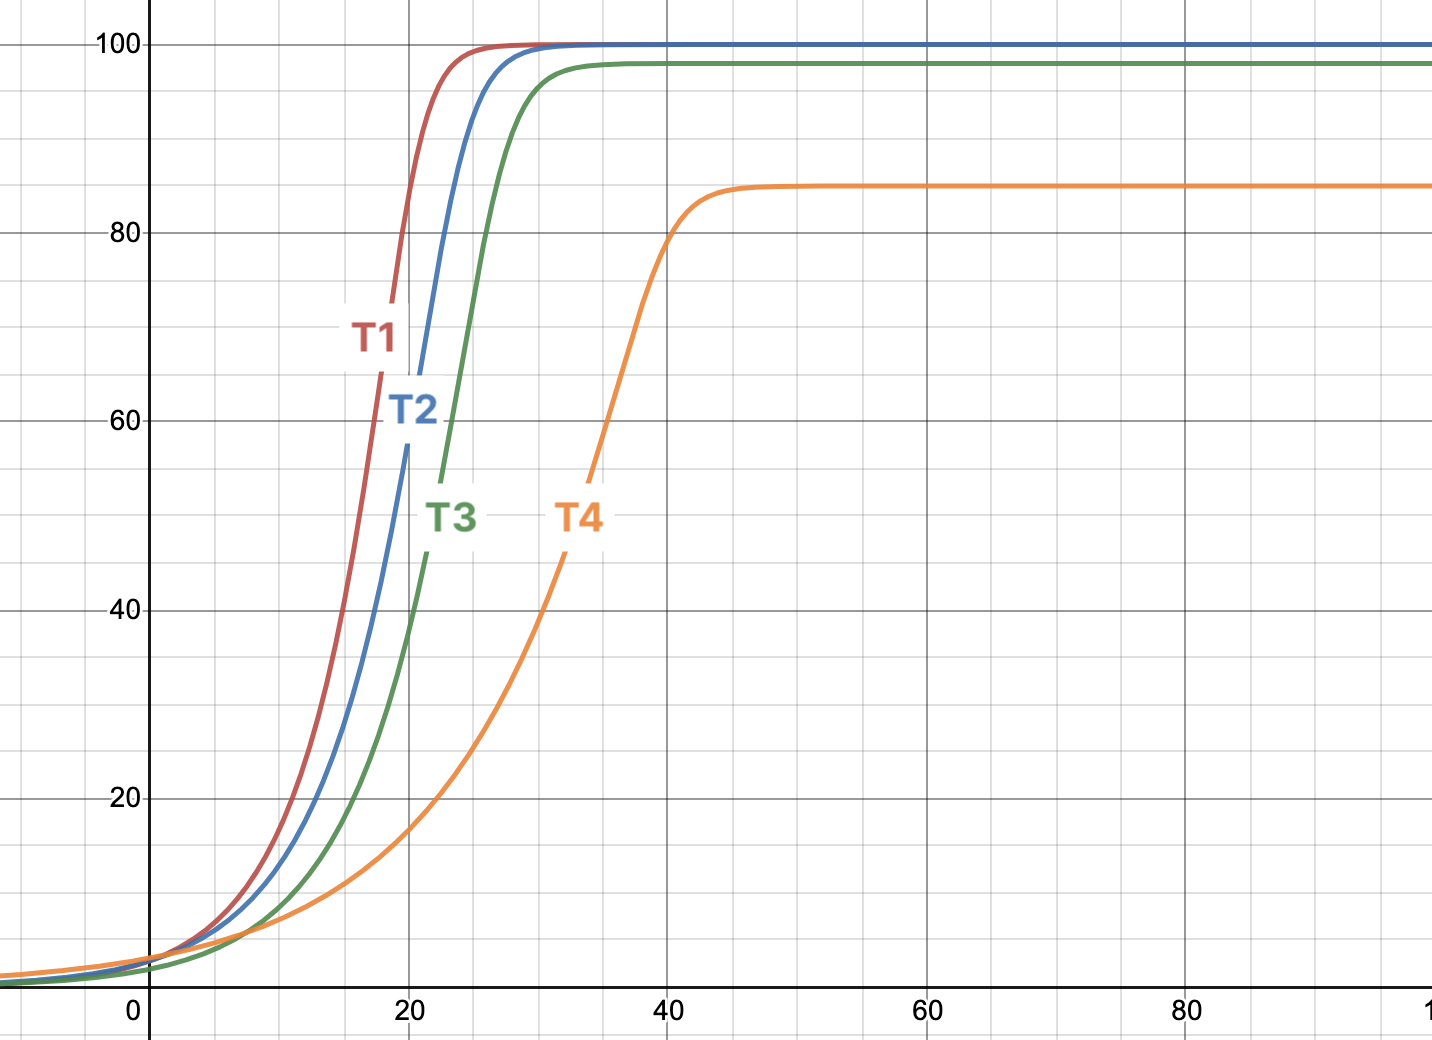
\includegraphics[width=10cm]{simGall.png}
    \caption{Summary of all simulation graphs from Test 1 to Test 4, superimposed over one another}
    \label{fig:simGall}
\end{figure}

\pagebreak
\section{Conclusion and Presentation}

\subsection{Advocacy Video and Script}

Note: This is the same script as used in the video submission. The script can be found at \url{https://docs.google.com/document/d/1-yg2IQCngEjx5vl-IGSysXytOATPMEbC1YStkj8K-xk}, and the video submission can be found at \url{https://drive.google.com/file/d/178F9aO_tx44gVPX-v5pAywAlJihySzU4}.

\subsubsection{Introduction}

Hello. We are a group of advocates from SST and we are here to discuss the importance of wearing masks and social distancing measures to prevent the spread of COVID-19.

According to the World Health Organisation, there have been about 128 million people worldwide infected with COVID-19 as of March 31 this year. Of this 128 million infections, there have been around 2.8 million deaths, putting the death rate at approximately 2.2%. 

Our project aims to find out whether social distancing and wearing of masks affects the spread of COVID-19 by mathematically modelling the issue through a computer simulation and real world data.

\subsubsection{Variables, Assumptions and Simplifications}
Before presenting our findings and model, here are our independent variables.

Firstly, there is the percentage of people who are wearing masks, which help reduce the number of droplets that may be inhaled when a person is exposed to a COVID-19 patient. 

Secondly, there is the percentage of the population that practices a 1m social distancing, which helps reduce the spread of the virus.

Here are our dependent variables.

Firstly, there is the total number of infections.

Secondly, there is the probability of an exposure becoming a new infection. 

Thirdly, there is the social exposure rate. This refers to the number of people that people are exposed to on a given day.

Next, there is the growth factor, g, which refers to the percentage change in the number of cases. 

The model also makes a few assumptions that may help define the model better.

It is assumed that the time before a person knows whether they are infected from a possible exposure is 2 weeks.

It is assumed that people wear their masks and do not remove masks throughout the pandemic when in close contact with other people.

It is assumed that people do not leave or enter the country, introducing and deporting cases.

It is assumed that at the start of the pandemic, only 1 case of COVID-19 is introduced into the community.

It is assumed that after a person has been infected and recovered from COVID-19, anti-bodies against the virus develop and thus the person is no longer susceptible to the virus and disease.

This calculation makes a few simplifications to remove the tediousness of the experimentation process.

Firstly, it is taken that the recovery time of the virus is approximately 2 weeks

Secondly, it is taken that all masks worn are the same and have an effectiveness of 50\% individually

Thirdly, the incubation period of COVID-19 is taken to be 14 days

Lastly, the strand of COVID-19 virus is the same

\subsubsection{Mathematical Model - Infections Function}

To aid in modelling the mathematical function, we go through a process of various functions that may be used in modelling the number of infections. Due to time, we will only present the final function used, a Richards’ Logistic Curve, that has 3 main features which may repeat.

The curve is defined based on the following, the flexibility of the curve, the epidemic size, the infection rate and the lag phase.

Initially, the graph is very similar to a exponential curve
Eventually, the gradient decreases and becomes constant at the inflection point for some time
Lastly, assuming no new clusters or outbreaks and continuous safe management measures, the infections should begin flattening and becoming constant
However, if a cluster of outbreak does occur again, certain sections of the curve may repeat itself, with the worst being another exponential-like increase

All real world data used is attributed to the CSSE at Johns Hopkins University and simulation data was created by ourselves

\subsubsection{Mathematical Model - Simulation Data}
To model the number of COVID-19 infected people, we came up with a simulation and ran 4 different scenarios with gathered data in graphs

In all the simulations, the constant parameters that are unchanged throughout the tests in the experimentation process are the original number of susceptible people, the original number of infected people, the recovery time of infected people, and the movement speed of people

The established base case for the comparison is the simulation Test 1, where no measures were practised

This is simulation Test 2, where only mask wearing was practised

This is simulation Test 3, where only social distancing was practised

This is simulation Test 4, where both social distancing and mask wearing was practised

Between Test 1 to Test 4, the independent factor that changed was not only the transmission rate but also the social distancing, which resulted in the slowest infection rate compared to the other 3 tests. With both of the factors affecting the infection rate combined, the infection rate reduced significantly.

\subsubsection{Mathematical Model - Real World Data}

In real life, the situation is not much different. In Singapore, social distancing and mask wearing was made mandatory upon the spread of COVID-19.

Here is the graph of the number of people in Singapore infected with COVID-19. This graph starts with a high rate of infection but caps out quickly when social distancing and mask wearing was made mandatory.

In India, the density of the population makes it difficult to practice social distancing. Poverty also makes it difficult to access masks. Here is the graph of the number of people in India infected with COVID-19. This graph has an increasing rate of infection.

In the United States, only a portion of the population practices social distancing and mask wearing. Here is the graph of the number of people in the United States infected with COVID-19. This graph has an increasing rate of infection.

\subsubsection{Conclusion}

From all the aforementioned mathematical models, we can tell that wearing masks and social distancing is effective in reducing the growth of COVID-19 cases.

For the simulation, the graphs for Test 2 and 3 were not as steep as the base case since people exclusively either wore masks or were socially distanced. However, in Test 4, when people both wore masks and socially distanced, the curve was much flatter, meaning the cases for a given period of time would be fewer and the cases at any point in time would not exceed potential hospital capacity.

This can also be seen mirrored in the real life data where Singapore’s curve flattened out much faster than the US or India.

The function used to graph these cases also showed a distinct exponential increase initially before SMM implementation, a slowly decreasing slope with an inflection point where the gradient is constant, finally slowly leveling off. The final leveling off is dependent on the time at which the SMM were implemented and the maximum infection size.

In conclusion, in order to “flatten the curve”,  we must all play our part in following the SMM put in place to ensure its timely success that would eventually lead to the maximum point of the curve where there are no more new infections.

\subsection{Flattening the Curve}

In order to “flatten the curve”, which can be seen in Figure \ref{fig:flattenCurve}, everyone must all play their part in following the safe management measures (SMM) that are put in place.

\begin{figure}[htbp]
    \centering
    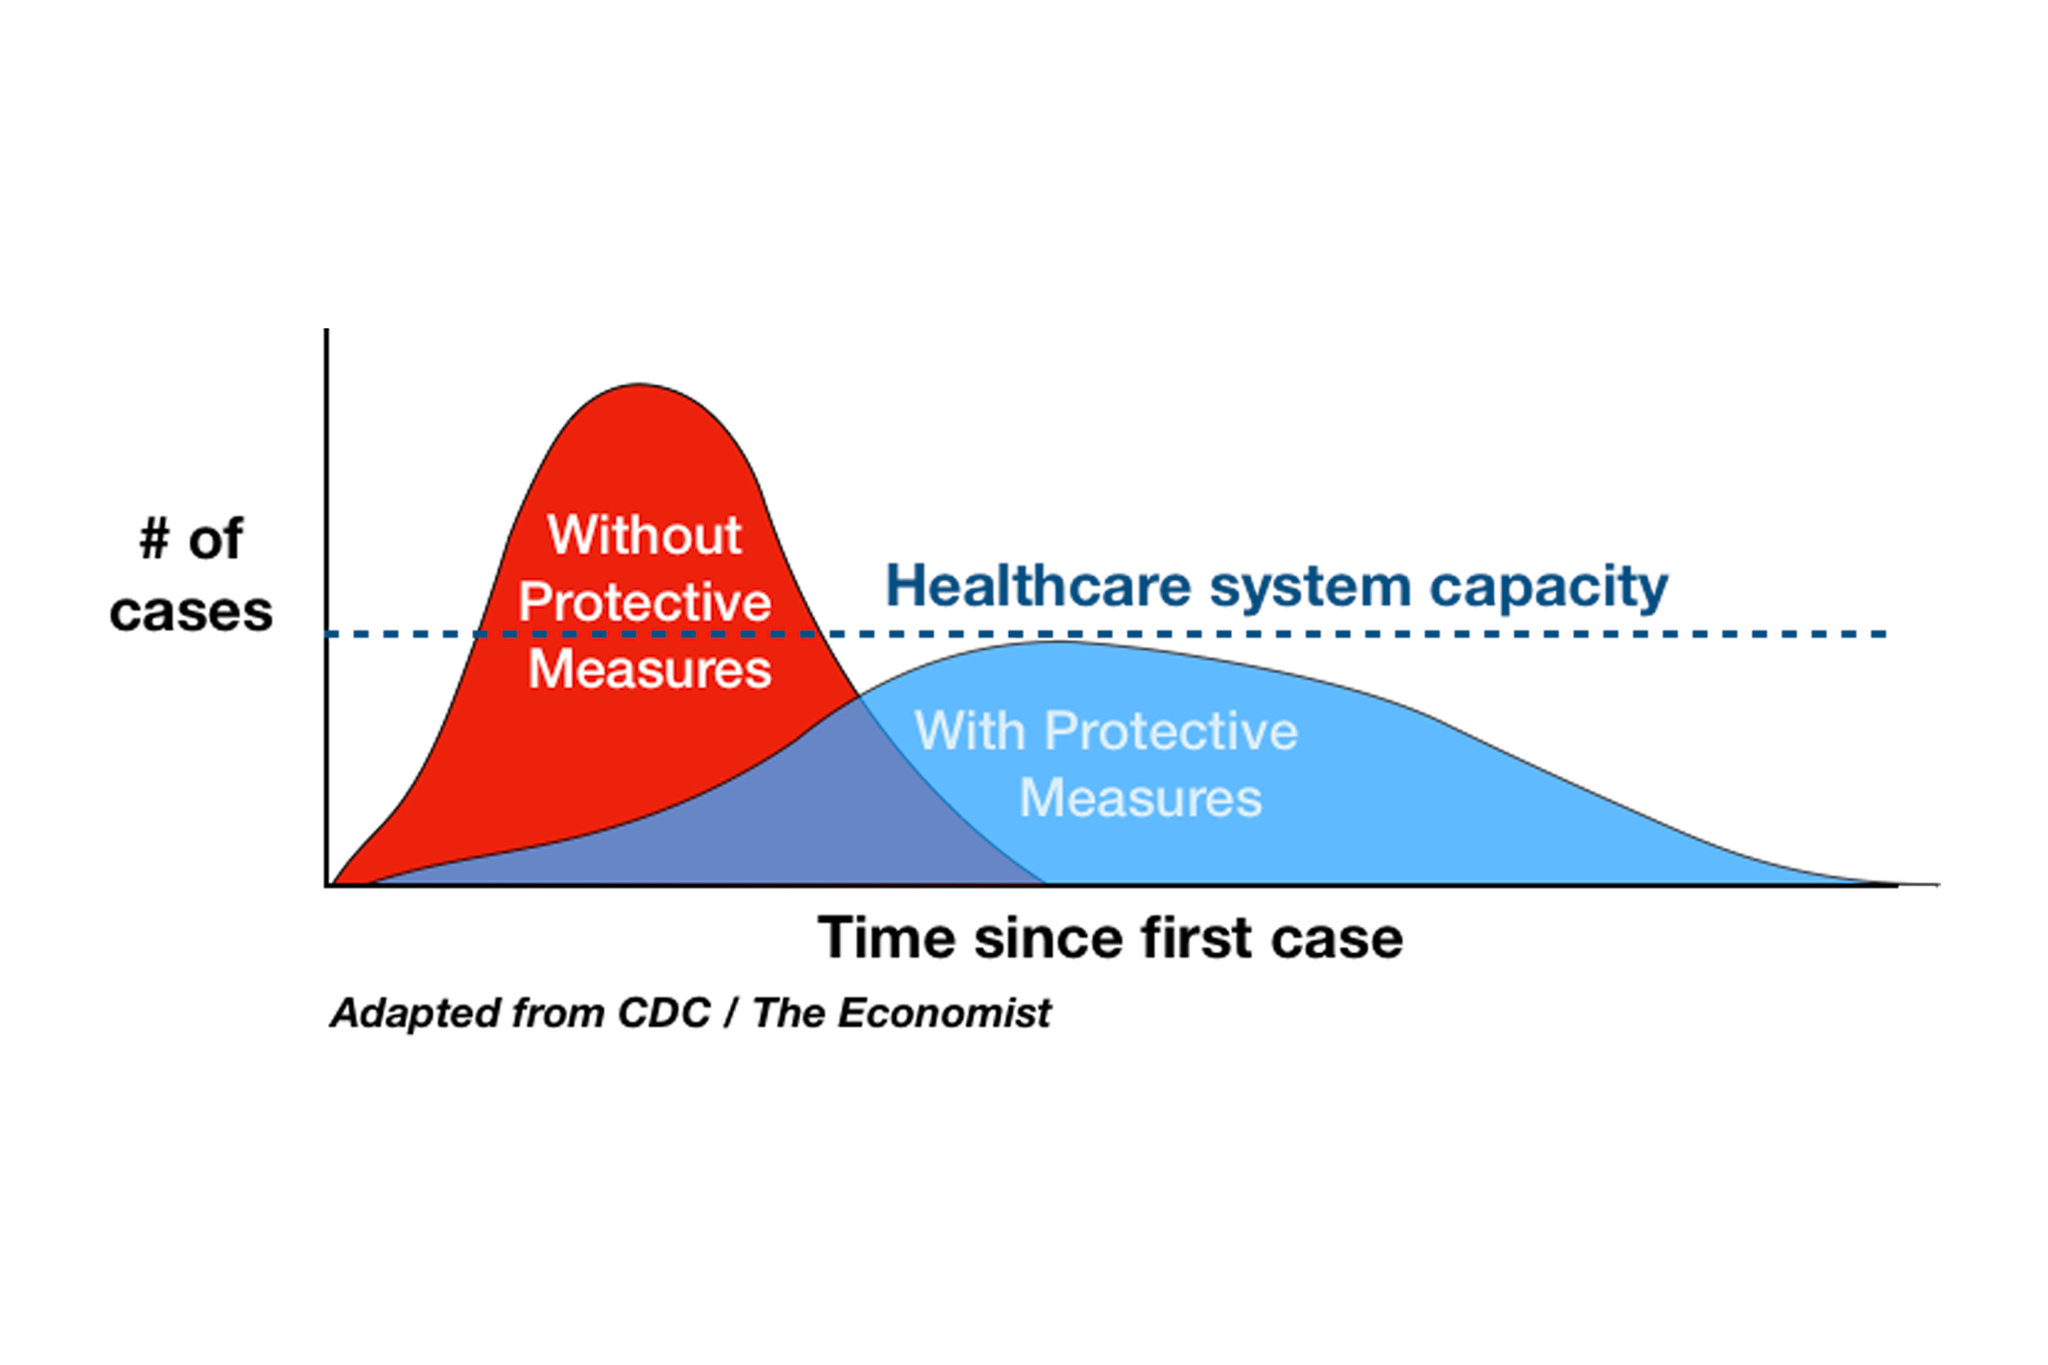
\includegraphics[width=10cm]{flattenCurve.jpg}
    \caption{Flattening the curve and its impacts, from \cite{flattencurve_roberts_2020}}
    \label{fig:flattenCurve}
\end{figure}

These include wearing of masks and social distancing, which together greatly help reduce the infection rate, ensuring its timely success, eventually leading to the maximum point of the curve where there are no more new infections to be lower.

The slower we reach the point where there are no more infections, the fewer cases there are at a given time. Hence, fewer hospitals will be used to treat COVID-19 cases and hospitals will be left for those with more serious diseases, and hospitals would be less likely to overflow.

\pagebreak
\bibliographystyle{plain}
\bibliography{references}
\end{document}
